% Main-text revision. Numerical results are retained from the frozen research record.
\documentclass[preprint,12pt]{elsarticle}
\usepackage[utf8]{inputenc}
\usepackage[T1]{fontenc}
\usepackage{amsmath,amssymb,amsfonts}
\usepackage{newtxtext,newtxmath}
\usepackage{booktabs,graphicx,array,url}
\usepackage[table]{xcolor}
\usepackage{microtype}
\usepackage{etoolbox}
\usepackage{tikz}
\usetikzlibrary{positioning,arrows.meta,calc}
\usepackage[section]{placeins}
\usepackage[hidelinks,hypertexnames=false]{hyperref}
\hypersetup{pdfauthor={Zixuan Liu},pdftitle={Support-conditioned prediction combination for few-shot battery state-of-health estimation under distribution shift}}
\journal{Journal of Energy Storage}
\newcommand{\R}{\mathbb{R}}
\newcommand{\figfile}[4]{\begin{figure}[!htbp]\centering\includegraphics[width=#2\columnwidth,height=.72\textheight,keepaspectratio]{#1}\caption{#3}\label{fig:#4}\end{figure}}
\setlength{\emergencystretch}{2em}
\makeatletter
% Keep the abstract and keywords together without reducing the text size.
\patchcmd{\pprintMaketitle}{\vskip36pt}{\vskip12pt}{}{\errmessage{Title spacing patch failed}}
\def\ps@pprintTitle{\let\@oddhead\@empty\let\@evenhead\@empty\def\@oddfoot{\hfil\thepage\hfil}\let\@evenfoot\@oddfoot}
\makeatother
% Consistent fixed type size; never stretch tables to fill the column.
\newcommand{\papertablesize}{\fontsize{9}{11}\selectfont}

% Align dedicated float pages at the top with a fixed gap between floats.
\makeatletter
\setlength{\@fptop}{0pt}
\setlength{\@fpsep}{18pt}
\setlength{\@fpbot}{0pt plus 1fil}
\makeatother

% Prefer figures/tables accompanied by text over sparsely filled float pages.
\renewcommand{\topfraction}{.9}
\renewcommand{\bottomfraction}{.8}
\renewcommand{\textfraction}{.1}
\renewcommand{\floatpagefraction}{.8}

\begin{document}
\begin{frontmatter}
\title{Support-conditioned prediction combination for few-shot battery state-of-health estimation under distribution shift}
\author[inst1]{Zixuan Liu\corref{cor1}}
\ead{2411621306@hbut.edu.cn}
\cortext[cor1]{Corresponding author: Zixuan Liu.}
\address[inst1]{Detroit Green Technology Institute, Hubei University of Technology, Wuhan 430068, China}
\begin{abstract}
  Battery state-of-health (SOH) estimation becomes challenging when the operating condition changes and only a small number of target labels are available. This study investigates current-query SOH estimation, in which each target cell provides ten early signal--capacity pairs and each subsequent query provides only its current partial-charge signal. We propose a support-conditioned Gaussian-process prediction-combination framework for combining source-based and target-conditioned estimates. The framework selects source experts according to their reference risks and further incorporates paired-waveform and conditional random-function predictions based on the early target support. On the XJTU, MATR and Tongji datasets, covering 365 cells and 21 held-out groups defined by conditions, batches, or protocols, the proposed method achieves MAEs of 2.6376, 1.9199 and 2.8508 SOH percentage points, respectively. These values correspond to reductions of 12.4\%, 28.5\% and 57.3\% compared with base GPR. The method also reduces MAE by 6.03\% across 50 cells in the frozen external evaluation on UL-PUR and MICH. These results demonstrate the effectiveness of support-conditioned prediction combination for few-shot SOH estimation under the evaluated operating conditions and information budget.
\end{abstract}
\begin{highlights}
\item A support-conditioned Gaussian-process framework is proposed for few-shot SOH estimation.
\item Ten early capacity labels guide source expert selection and target conditioning.
\item Current partial-charge signals enable query-level SOH estimation under distribution shift.
\item MAE reductions of 12.4\%, 28.5\% and 57.3\% are achieved on XJTU, MATR and Tongji.
\item Frozen external evaluation shows a 6.03\% MAE reduction across 50 cells.
\end{highlights}
\begin{keyword}
Lithium-ion battery \sep State-of-health estimation \sep Few-shot adaptation \sep Gaussian process regression \sep Prediction combination \sep Operating-condition shift
\end{keyword}
\end{frontmatter}

\section{Introduction}
\label{sec:introduction}
Accurate battery state-of-health (SOH) estimation supports capacity monitoring, maintenance planning and battery-management decisions \citep{berecibar2016,waag2014,farmann2015}. Estimating SOH from partial-charge signals can reduce the need for a complete charge--discharge record at every query \citep{wang2024}. In practice, however, a target cell may differ from the source cells in operating condition, charging protocol, battery type or ageing history. These differences can change the relationship between charging signals and available discharge capacity \citep{ecker2012,waldmann2014,dubarry2012}, making direct transfer from source data unreliable.

A small number of target-cell labels can provide useful information for adaptation, but how these labels should be used remains unclear. Existing transfer methods commonly use unlabelled target data for domain alignment or fine-tune a pretrained model on a target dataset. Their measurement requirements, target-label budgets and prediction tasks are not the same. A practical battery setting is one in which a target cell provides only a few early capacity measurements, while each later query provides its current partial-charge signal. The model must therefore use source knowledge together with the early target observations, without using the capacity label of the current query.

This study investigates current-query SOH estimation under this setting. Each target cell provides ten eligible early signal--capacity pairs as a support set. For every subsequent query, voltage, current and elapsed-time signals from the current partial-charge segment are available, whereas the corresponding capacity label is used only for final error calculation. The task is different from forecasting an entire future degradation trajectory from early observations alone, because the current query signal remains available at prediction time. The early support can both provide an individual reference for the target cell and indicate which source predictions are more suitable for it.

We propose a support-conditioned Gaussian-process prediction-combination framework to address this problem. The framework first learns a source representation and uses the similarity and reference risk of source episodes to select and aggregate candidate source predictions. It then uses the same target support to construct two additional estimates: a paired-waveform branch compares the current charging waveform with the target cell's early waveforms, while a conditional random-function branch models within-cell SOH variation conditioned on the support labels. The source-based and target-conditioned estimates are expressed on a common SOH scale and combined for the final query prediction. Thus, the early support contributes both to source-expert selection and to target-conditioned prediction without exposing later query labels.

The contributions of this study are as follows:
\begin{enumerate}
\item We formulate current-query SOH estimation as a support-conditioned prediction-combination problem with a fixed ten-label information boundary.
\item We develop a Gaussian-process framework that connects source-expert selection with target-conditioned waveform and function predictions, and evaluate the roles of these components under a common information budget.
\item We conduct cell-disjoint development evaluations across 365 cells and 21 held-out groups defined by conditions, batches, or protocols, followed by a frozen external evaluation on the previously unused UL-PUR and MICH datasets.
\end{enumerate}

\section{Related work}
\label{sec:related}
\subsection{Data-driven and partial-charge SOH estimation}
Data-driven SOH estimators learn a relationship between measurable battery behaviour and capacity using either designed indicators or learned signal representations. Reviews of battery monitoring and capacity estimation emphasize that the available measurements and operating conditions determine which relationships can be exploited \citep{berecibar2016,waag2014,farmann2015}. For partial-charge estimation, the measurement window and feature representation are therefore closely linked to the estimator design.

Previous studies have extracted health information from voltage relaxation, short charging segments or partial charging curves. Zhu et al.\ \citep{zhu2022} use statistical features from voltage relaxation after full charging, Wang et al.\ \citep{wang2024} combine features from a short charging segment with learned degradation dynamics in a physics-informed neural network, and Lu et al.\ \citep{lu2023} learn charging representations for cross-domain estimation. Partial charging voltage profiles have also been used directly, with studies focusing on informative voltage ranges and data-driven feature construction \citep{stroe2018,meng2019,tang2024}. These studies show that restricted charging measurements contain useful information about battery health, but their inputs and adaptation procedures differ.

The prediction target is also important. Severson et al.\ \citep{severson2019} use early-cycle information to predict cycle life, whereas a current-query SOH estimator continues to receive measurements at the time being evaluated. The present study belongs to the latter setting: it uses the current partial-charge voltage, current and elapsed-time signals together with ten early capacity labels. Its comparisons therefore concern measurement-conditioned SOH estimation under held-out groups, rather than lifetime forecasting from early observations alone.

\subsection{Transfer learning and few-shot battery adaptation}
Transfer learning addresses changes between source and target distributions by reusing source data or source model parameters \citep{pan2010}. Existing approaches include feature alignment, domain-adversarial learning, transfer-based fine-tuning and meta-learning. Feature-alignment methods reduce discrepancies between source and target representations, as in deep adaptation networks and correlation alignment \citep{long2015,sun2016}, while domain-adversarial training learns features that support prediction while reducing domain information \citep{ganin2016}. In battery estimation, Lu et al.\ \citep{lu2023} combine estimator selection with adaptation using labelled source samples and unlabelled target signals.

When target labels are available, a pretrained estimator can be updated using a smaller target dataset. Zhu et al.\ \citep{zhu2022} use transfer learning to accommodate changes in voltage-relaxation features across batteries and cycling conditions. Meta-learning instead trains across tasks to facilitate subsequent adaptation \citep{finn2017}. For battery SOH estimation, Zhao et al.\ \citep{zhao2025} evaluate a CNN--attention meta-learning method using six cycles from a target battery across battery types and temperatures. These approaches demonstrate different ways of using target information, but their measurement modalities, label budgets and prediction tasks are not directly equivalent.

The present study fixes the source representation after source training, provides ten eligible early target labels and allows only the current partial-charge signal at a later query. It therefore examines source-expert selection and target conditioning under a common few-shot information budget. Published errors from other adaptation protocols are used as contextual evidence rather than as additional entries in the matched comparison.

\subsection{Gaussian processes and conditional prediction}
Gaussian-process regression (GPR) models a distribution over functions through a mean function and a covariance function. For fixed covariance parameters, conditioning on labelled observations gives a closed-form posterior prediction \citep{rasmussen2006,mackay1998}. This separates learning a source relationship from updating a prediction with a small labelled support set, making GPR useful for sparse-label adaptation. Battery studies have used GPR with physical-model features, hierarchical feature construction and partial-charge reconstruction for SOH estimation \citep{lyu2020,jin2023,xiong2023}.

GP-based battery studies include capacity estimation, temporal prognosis and function combination. Liu et al.\ \citep{calce_gp2013}, for example, use a combination linear GP functional regression model to describe global capacity decline together with local regeneration. Yu et al.\ \citep{yu2018} combine multiscale regression and GPR to separate global degradation from local fluctuations. Such work demonstrates the usefulness of combining GP components for battery prognosis, whereas the present study conditions each current-query SOH estimate on an observed partial-charge signal and early target support.

Prediction combination can improve robustness when different predictors respond differently to a distribution shift. Within the proposed framework, source leave-out performance supplies the reference risk used to select or aggregate transferred predictions, while covariance-based conditioning constructs target estimates from the support observations. The same support also anchors the paired-waveform representation. The contribution of this study is therefore an experimental organization of established representation, selection and GP-conditioning components under one information budget, rather than a new GP principle. Matched waveform replacements, simpler functional alternatives and the complete module combinations are used to examine the roles of these components.

\section{Proposed method}
\label{sec:method}
The proposed method combines source-based and target-conditioned predictions under a common support budget. The source-based path learns a transferable prediction and determines which source experts are suitable for a target cell. The target-conditioned paths use the same early support and the current query waveform to construct complementary estimates. We first define the information available at prediction time and give an overview of the framework, then describe the two prediction paths and their final combination.
\subsection{Problem formulation and framework overview}
For cell $c$, let $x_{ci}\in\R^{3\times128}$ contain interpolated voltage, current and elapsed time from a qualified partial-charge segment. Let $q_{ci}$ be the associated measured discharge capacity. The SOH label and early support set are
\begin{equation}
y_{ci}=q_{ci}/q_{c1},\qquad S_c=\{(x_{ci},y_{ci})\}_{i=1}^{K},\quad K=10.
\end{equation}
The reference $q_{c1}$ is the first qualified capacity measurement; it need not equal the nominal capacity. SOH values above one are retained. For a later query $j>K$, the estimator has the form
\begin{equation}
\widehat y_{cj}=F(D_s,S_c,x_{cj};\theta_s),
\label{eq:permission}
\end{equation}
where $D_s$ is the permitted source information and $\theta_s$ is fitted source state. Figure~\ref{fig:permission} separates the information used for source fitting, target prediction and evaluation. Query labels, future signals and the complete query population are unavailable to the prediction procedure. The early reference capacity itself supplies target information, so a source-only predictor under this normalization is not a zero-target-information method.

Starting from the base GPR, the prediction flow has three stages. First, source representation learning (M1) constructs the modelling space and determines how the early support enters the source prediction. Second, reference-risk expert selection (M2) uses the target cell's early signals to select and aggregate suitable source experts. These two modules form the source-based prediction $p_{B12}$. Third, the paired-waveform branch (M3) and conditional random-function branch (M4) use the same support to produce additional estimates, denoted by $q_3$ and $q_4$. Figure~\ref{fig:architecture} shows the successive combination of these estimates. Each branch produces an independent SOH estimate; it is not trained to predict the residual of its parent model. We denote the base GPR by B and the progressive configurations by B1, B12, B123 and B1234; the digits identify the included modules.

\begin{figure}[!htbp]\centering
\resizebox{.92\columnwidth}{!}{% Publication-style vector diagram: information boundary and evaluation flow.
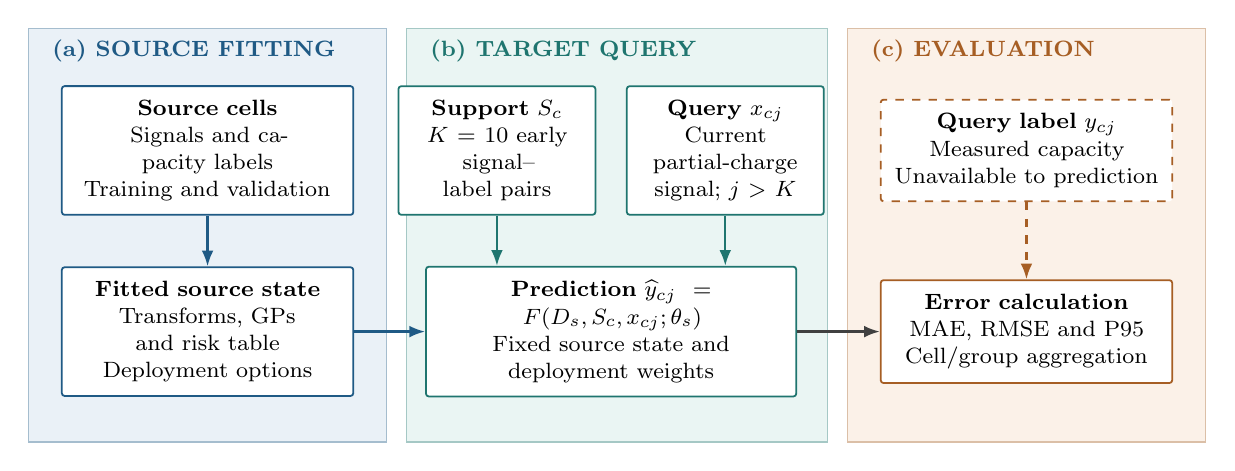
\begin{tikzpicture}[x=1cm,y=1cm,font=\fontsize{8.2}{9.8}\selectfont,align=center,
  box/.style={draw=black!55,line width=.65pt,fill=white,inner sep=5pt,rounded corners=1pt},
  arr/.style={-{Latex[length=2mm]},line width=.85pt,draw=black!75},
  hdr/.style={font=\bfseries\fontsize{8.5}{10}\selectfont,anchor=west},
  small/.style={font=\fontsize{7.4}{8.8}\selectfont,text=black!72}]
\definecolor{navy}{HTML}{1F5A85}
\definecolor{teal}{HTML}{1F756F}
\definecolor{orange}{HTML}{A65E24}
\definecolor{lightblue}{HTML}{EAF1F7}
\definecolor{lightteal}{HTML}{EAF5F3}
\definecolor{lightorange}{HTML}{FBF1E8}
\fill[lightblue] (0,0) rectangle (4.55,-5.25);
\fill[lightteal] (4.8,0) rectangle (10.15,-5.25);
\fill[lightorange] (10.4,0) rectangle (14.95,-5.25);
\draw[navy!40,line width=.55pt] (0,0) rectangle (4.55,-5.25);
\draw[teal!40,line width=.55pt] (4.8,0) rectangle (10.15,-5.25);
\draw[orange!40,line width=.55pt] (10.4,0) rectangle (14.95,-5.25);
\node[hdr,text=navy] at (.18,-.28) {(a) SOURCE FITTING};
\node[hdr,text=teal] at (4.98,-.28) {(b) TARGET QUERY};
\node[hdr,text=orange] at (10.58,-.28) {(c) EVALUATION};
\node[box,draw=navy,text width=3.35cm,minimum height=1.05cm] (src) at (2.275,-1.55)
  {\textbf{Source cells}\\Signals and capacity labels\\Training and validation};
\node[box,draw=navy,text width=3.35cm,minimum height=1.05cm] (fit) at (2.275,-3.85)
  {\textbf{Fitted source state}\\Transforms, GPs and risk table\\Deployment options};
\draw[arr,draw=navy] (src)--(fit);
\node[box,draw=teal,text width=2.15cm,minimum height=1.18cm] (sup) at (5.95,-1.55)
  {\textbf{Support }$S_c$\\$K=10$ early\\signal--label pairs};
\node[box,draw=teal,text width=2.15cm,minimum height=1.18cm] (qry) at (8.85,-1.55)
  {\textbf{Query }$x_{cj}$\\Current partial-charge\\signal; $j>K$};
\node[box,draw=teal,text width=4.35cm,minimum height=1.08cm] (pred) at (7.4,-3.85)
  {\textbf{Prediction }$\widehat y_{cj}=F(D_s,S_c,x_{cj};\theta_s)$\\Fixed source state and deployment weights};
\draw[arr,draw=navy] (fit.east)--(pred.west);
\draw[arr,draw=teal] (sup.south)--(sup.south |- pred.north);
\draw[arr,draw=teal] (qry.south)--(qry.south |- pred.north);
\node[box,draw=orange,dashed,text width=3.35cm,minimum height=1.18cm] (truth) at (12.675,-1.55)
  {\textbf{Query label }$y_{cj}$\\Measured capacity\\Unavailable to prediction};
\node[box,draw=orange,text width=3.35cm,minimum height=1.08cm] (eval) at (12.675,-3.85)
  {\textbf{Error calculation}\\MAE, RMSE and P95\\Cell/group aggregation};
\draw[arr,draw=orange,dashed] (truth)--(eval);
\draw[arr] (pred.east)--(eval.west);
\end{tikzpicture}
}
\caption{Task and information boundary. Source fitting, target prediction and evaluation are separated. The first ten eligible target measurements and the current query signal enter prediction; the query capacity label enters error calculation only. Development scores informed architecture and global-strength selection, whereas the subsequent UL-PUR and MICH evaluations used frozen XJTU models and weights.}\label{fig:permission}
\end{figure}

\begin{figure}[!htbp]\centering
\resizebox{.92\columnwidth}{!}{% Shared style with Figure 1; solid arrows carry predictions, dashed arrows inputs.
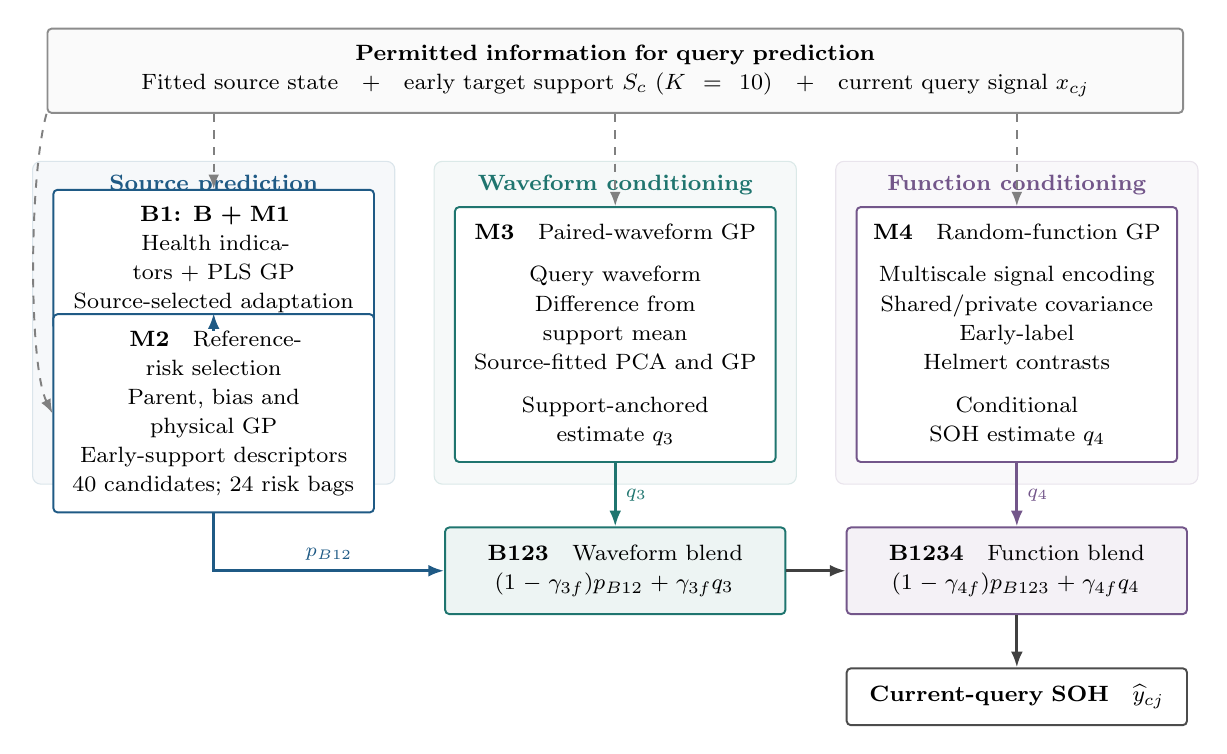
\begin{tikzpicture}[x=1cm,y=1cm,font=\fontsize{8.5}{10.5}\selectfont,align=center,
 box/.style={draw=black!45,line width=.7pt,rounded corners=1.5pt,fill=white,inner sep=6pt},
 flow/.style={-{Latex[length=2mm]},line width=1pt,draw=black!75},
 info/.style={-{Latex[length=1.8mm]},line width=.7pt,dashed,draw=black!50},
 note/.style={font=\fontsize{7.5}{9}\selectfont,text=black!70}]
\definecolor{srcblue}{HTML}{1F5A85}
\definecolor{targetgreen}{HTML}{1F756F}
\definecolor{funcpurple}{HTML}{73568A}
\node[box,fill=black!2,text width=14cm,minimum height=.9cm] (inputs) at (7.45,.3)
 {\textbf{Permitted information for query prediction}\\Fitted source state\quad +\quad early target support $S_c$ ($K=10$)\quad +\quad current query signal $x_{cj}$};
\fill[srcblue!4,draw=srcblue!16,line width=.4pt,rounded corners=3pt] (.05,-.85) rectangle (4.65,-4.95);
\fill[targetgreen!4,draw=targetgreen!16,line width=.4pt,rounded corners=3pt] (5.15,-.85) rectangle (9.75,-4.95);
\fill[funcpurple!4,draw=funcpurple!16,line width=.4pt,rounded corners=3pt] (10.25,-.85) rectangle (14.85,-4.95);
\node[font=\fontsize{8.5}{10.5}\selectfont\bfseries,text=srcblue] at (2.35,-1.15) {Source prediction};
\node[font=\fontsize{8.5}{10.5}\selectfont\bfseries,text=targetgreen] at (7.45,-1.15) {Waveform conditioning};
\node[font=\fontsize{8.5}{10.5}\selectfont\bfseries,text=funcpurple] at (12.55,-1.15) {Function conditioning};
\node[box,draw=srcblue,text width=3.65cm,minimum height=1.05cm] (m1) at (2.35,-2.1)
 {\textbf{B1: B + M1}\\Health indicators + PLS GP\\Source-selected adaptation};
\node[box,draw=srcblue,text width=3.65cm,minimum height=1.2cm] (m2) at (2.35,-4.05)
 {\textbf{M2}\quad Reference-risk selection\\Parent, bias and physical GP\\Early-support descriptors\\40 candidates; 24 risk bags};
\draw[flow,draw=srcblue] (m1)--(m2);
\node[box,draw=targetgreen,text width=3.65cm,minimum height=2.35cm] (m3) at (7.45,-3.05)
 {\textbf{M3}\quad Paired-waveform GP\\[5pt]Query waveform\\Difference from support mean\\Source-fitted PCA and GP\\[5pt]Support-anchored estimate $q_3$};
\node[box,draw=funcpurple,text width=3.65cm,minimum height=2.35cm] (m4) at (12.55,-3.05)
 {\textbf{M4}\quad Random-function GP\\[5pt]Multiscale signal encoding\\Shared/private covariance\\Early-label Helmert contrasts\\[5pt]Conditional SOH estimate $q_4$};
\draw[info] (inputs.south -| m1.north)--(m1.north);
\draw[info] (inputs.south west) .. controls (.00,-1.05) and (.00,-3.45) .. (m2.west);
\draw[info] (inputs.south -| m3.north)--(m3.north);
\draw[info] (inputs.south -| m4.north)--(m4.north);
\node[box,draw=targetgreen,fill=targetgreen!8,text width=3.9cm,minimum height=1.1cm] (blend3) at (7.45,-6.05)
 {\textbf{B123}\quad Waveform blend\\$(1-\gamma_{3f})p_{B12}+\gamma_{3f}q_3$};
\node[box,draw=funcpurple,fill=funcpurple!8,text width=3.9cm,minimum height=1.1cm] (blend4) at (12.55,-6.05)
 {\textbf{B1234}\quad Function blend\\$(1-\gamma_{4f})p_{B123}+\gamma_{4f}q_4$};
\draw[flow,draw=srcblue] (m2.south)--(2.35,-6.05)--node[above,note,text=srcblue] {$p_{B12}$} (blend3.west);
\draw[flow,draw=targetgreen] (m3.south)--node[right,note,text=targetgreen] {$q_3$} (blend3.north);
\draw[flow,draw=funcpurple] (m4.south)--node[right,note,text=funcpurple] {$q_4$} (blend4.north);
\draw[flow] (blend3.east)--(blend4.west);
\node[box,draw=black!70,text width=3.9cm,minimum height=.65cm] (out) at (12.55,-7.65)
 {\textbf{Current-query SOH}\quad $\widehat y_{cj}$};
\draw[flow] (blend4)--(out);
% Blending and arrow conventions are defined in the caption and equations;
% the diagram retains only the prediction flow and permitted inputs.
\end{tikzpicture}
}
\caption{Support-conditioned prediction combination. M1 and M2 form the source-prediction path. M3 and M4 each produce an SOH estimate from source-fitted state, early target support and the current query; these estimates are successively blended with the parent prediction. Solid arrows carry predictions and dashed arrows indicate input information. The branch estimates are not fitted to parent-model residuals.}\label{fig:architecture}
\end{figure}

\subsection{Source-based prediction path}
The source-based path addresses the question of which information learned from the source data should be transferred to the target cell. It begins with a compact indicator-based GPR and then adds a source-supervised representation and a reference-risk selection step.
\subsubsection{Base GPR and source representation learning}
The base predictor uses summary indicators, whereas M1 adds source-supervised combinations of these indicators while retaining the original coordinates. The resulting representation is fitted only on source data. Target support is used at prediction time through a source-selected adaptation mode, rather than by refitting the feature transformation.

\paragraph{Base predictor.}
The base model uses 21 health indicators: the mean, standard deviation, minimum, maximum, first value, last value and linear slope of each signal channel. A source-fitted scaler precedes an RBF-plus-white-noise GP. Its source posterior mean is
\begin{equation}
p_B(x)=\mu_s+k(x,X_s)[K_s+\sigma_n^2I]^{-1}(y_s-\mu_s),
\end{equation}
with predictions transformed back to the original SOH scale. B uses the source-only mode and does not perform an additional target posterior update.

\paragraph{Source representation and adaptation.}
M1 prunes constant or redundant indicator dimensions and learns a supervised partial-least-squares (PLS) projection using source training labels. The retained standardized indicators and their PLS scores are concatenated to form the GP input. PLS supplies source-supervised combinations; concatenation retains indicator coordinates alongside them. Source validation selects 2, 4 or 8 PLS components and one of three adaptation modes: source-only prediction, support-mean bias correction or GP posterior conditioning. For bias correction,
\begin{equation}
p_{\rm bias}(x)=p_s(x)+b_c,\qquad b_c=\frac{1}{K}\sum_{i=1}^K[y_{ci}-p_s(x_{ci})].
\end{equation}
For posterior conditioning, source-posterior covariances update the query mean using the same support residuals. Neither the scaler nor PLS loadings are refitted on the target. M1 therefore evaluates a representation together with a source-selected adaptation mode, rather than an isolated representation change.

\subsubsection{Reference-risk expert selection}
M2 addresses the possibility that different source predictions respond differently to a distribution shift. It uses source reference errors to estimate which candidate prediction is more suitable for the current target cell. Its calculation has three stages: construct candidate experts, estimate their target-relevant risks from source leave-out episodes, and aggregate the selected experts across risk resamples.

\paragraph{Candidate experts.} A physical-feature GP uses charge-derived and waveform-shape features as an alternative to the parent prediction. It is an empirical regressor. An expert indexed by $e=(\beta_e,w_e)$ produces
\begin{equation}
p_e(x)=(1-w_e)\{p(x)+\beta_e b_c\}+w_e p_{\rm phys}(x),
\end{equation}
where $p$ is the permitted parent and $b_c$ its support-mean residual. The expert grid uses $\beta_e\in\{-1,-0.5,-0.25,0,0.25,0.5,0.75,1\}$ and $w_e\in\{0,0.25,0.5,0.75,1\}$, giving 40 candidate combinations.

The physical view has twelve entries. Trapezoidal integration of measured current over elapsed time gives the window charge $Q_w$ in Ah. The entries are $Q_w/q_{c1}$, mean current divided by $q_{c1}$, current standard deviation divided by mean current, initial voltage, voltage span, and seven relative voltages sampled at equally spaced cumulative-charge fractions from 0.125 to 0.875. Relative voltage is measured from the window start and divided by its voltage span. These are observed charging descriptors, not an electrochemical capacity model.

\paragraph{Source reference table and target-relevant risk.}
Source leave-out episodes provide an error table indexed by reference episode and expert. Let $E_{re}$ be the MAE of expert $e$ on source reference episode $r$. Each reference descriptor concatenates the mean and standard deviation of each health indicator over the first ten eligible measurements. Source-fitted pruning, domain-weighted standardization and an eight-component weighted PCA produce the reference descriptor $z_r$ and target descriptor $z_c$. Write $d_r=\|z_r-z_c\|^2/\dim(z_c)$. Reference weights initially give equal mass to source domains and equal mass to cells within a domain. In bag $b$, references are resampled with replacement within each domain, preserving its reference count; the resulting normalized multiplicities are $a_r^{(b)}$. Then
\begin{align}
\ell_r^{(b)}&=\frac{a_r^{(b)}\exp[-d_r/(2h^2)]}{\sum_u a_u^{(b)}\exp[-d_u/(2h^2)]},\\
\widehat R_e^{(b)}&=\sum_r\big[(1-\eta)a_r^{(b)}+\eta\ell_r^{(b)}\big]E_{re}.
\end{align}
The bandwidth $h$ controls how strongly descriptor distance affects locality, and $\eta$ balances local and domain-weighted reference errors. This estimates risk from source references, not from the unknown target-query label. The same weights produce RMSE and P95 tie-breakers. Source validation selects $h\in\{0.25,1,4\}$ and $\eta\in\{0.5,1\}$; the 24 draws use seeds 0--23. Reference labels belong to source episodes, whereas the target descriptor uses only its early signals. No target-query errors enter the risk table.

\paragraph{Expert selection and aggregation.}
For each of 24 bagged risk-weight draws, the expert with the lowest MAE is selected, with RMSE and P95 as tie-breakers:
\begin{equation}
e_b=\mathop{\arg\min}_{e}\widehat R_e^{(b)}(S_c),\qquad
p_{B12}(x)=\frac{1}{24}\sum_{b=1}^{24}p_{e_b}(x).
\end{equation}
With B1 as the parent, this aggregation gives B12; the same rule uses the permitted parent in other module subsets. The reported M2 is the frozen v3 configuration. The risk setting is source-selected and fixed for deployment. The mechanism selects from a discrete expert table; 24 risk bags do not require training 24 additional GPs.

\subsection{Target-conditioned prediction paths}
The target-conditioned paths address a different question: how can the target cell's early behaviour modify a current-query estimate? Both paths use the same ten-label support, but they represent target information differently. M3 focuses on waveform changes relative to an early target reference, whereas M4 models within-cell SOH variation as a conditional function.
\subsubsection{Support-conditioned waveform prediction}
Summary indicators compress each charge segment into a small set of statistics. M3 retains information beyond these summaries by pairing the current waveform with its change from an early target reference. This construction emphasizes within-cell waveform variation before estimating the current SOH.

\paragraph{Paired representation.}
For each waveform, voltage is shifted by 3.5 V, current is divided by $q_{c1}$ in Ah, and elapsed time is shifted to the segment start and divided by 3,600. Flattening gives $u_{ci}\in\R^{384}$, and the paired input is $[u_{ci},u_{ci}-K^{-1}\sum_{j\leq K}u_{cj}]$. Dimensions with source standard deviations no larger than $10^{-6}$, $10^{-4}$ and $10^{-7}$ in the voltage, current and time blocks are removed before standardization. PCA scores with standard deviation no larger than $10^{-6}$ are discarded; retained scores are standardized again using source data only.

\paragraph{Relative-SOH prediction and target anchoring.}
The branch GP is trained on source SOH relative to each source cell's early-support mean. Source validation selects support-mean bias correction or posterior conditioning to obtain the target estimate $q_3(x,S_c)$. This formulation relates current waveform changes to relative SOH and uses the target support to restore its level. The output $q_3(x,S_c)$ is an SOH estimate that is subsequently blended with the parent prediction; its training target is not the parent prediction error. The paired/absolute controls evaluate whether the reference pairing helps under matched settings.

\paragraph{Source fitting settings.}
The source GP candidates use a constant-amplitude RBF or Mat\'ern-$3/2$ kernel plus white noise. Initial signal variance, length scale and noise variance are 1, 1 and 0.01, with bounds $[10^{-3},10^3]$, $[10^{-2},10^3]$ and $[10^{-6},1]$, respectively. Before marginal-likelihood fitting, the source-relative labels are standardized using their source mean and standard deviation. Predictions are transformed back to the relative SOH scale before the target early-support level is added. Kernel and adaptation-mode choices use source validation.

\subsubsection{Conditional random-function prediction}
M4 provides a second target-conditioned estimate by modelling within-cell SOH contrasts in a multiscale signal representation. The shared covariance term captures structure common to source cells, while the private term permits additional dependence within a target cell. Support contrasts update the functional prediction, and an anchor restores its absolute SOH level.

\paragraph{Multiscale signal representation.}
The encoder applies five orthonormal Haar decomposition levels to the normalized signals defined for M3. It concatenates the level-five approximation, signed level-five and level-four details, and four local root-mean-square energies for each of the first three detail levels. The resulting 84 features are paired with their differences from the early-support mean. Source standardization and eight-component PCA, followed by latent standardization, produce $z$. Raw and latent standard-deviation thresholds are $10^{-7}$ and $10^{-6}$.

\paragraph{Source contrast model.}
For encoded observations $z_i$ from cells $c_i$, the covariance is
\begin{equation}
C_{ij}=k_s(z_i,z_j)+\rho\,\mathbf{1}(c_i=c_j)k_p(z_i,z_j)+\sigma_n^2\mathbf{1}(i=j),\qquad\rho\geq0.
\label{eq:m4cov}
\end{equation}
The shared term represents structure across cells, while the private term permits additional within-cell dependence. The private covariance uses the fitted signal-kernel structure. A block contrast matrix $H_s$ removes source cell intercepts; source likelihood fitting uses $H_sCH_s^{\mathsf T}$ and the corresponding label contrasts. This shared/private construction is a standard functional modelling device; its contribution here is evaluated experimentally.

For clarity, the following expressions are in the fitted contrast scale, with labels $\widetilde y=y/s_y$, where $s_y$ is the source contrast root-mean-square scale. Let $A=H_sCH_s^{\mathsf T}$ and $U(z)=k_s(z,Z_s)H_s^{\mathsf T}$. The source-conditioned mean and target latent covariance are
\begin{align}
m(z)&=U(z)A^{-1}H_s\widetilde y_s,\\
V(z,z')&=k_s(z,z')-U(z)A^{-1}U(z')^{\mathsf T}+\rho k_p(z,z').
\end{align}
\paragraph{Target conditioning and SOH restoration.}
For the target, $K-1$ Helmert contrasts of the first ten labels condition the functional prediction. A support-mean anchor restores the absolute SOH level, producing $q_4(x,S_c)$. M4 is fitted to source SOH contrasts rather than the residuals of B123. Shared-function and shared/private-slope replacements test whether the chosen covariance structure is necessary for the observed gains.

The private term applies within the new target cell and has no cross-covariance with source cells. Let $Z_c$ denote the ten support representations, and let $H$ be the $(K-1)\times K$ Helmert matrix, satisfying $H\mathbf{1}=0$ and $HH^{\mathsf T}=I$. With $m_c=m(Z_c)$ and $V_{cc}=V(Z_c,Z_c)$,
\begin{align}
\omega_c&=[H(V_{cc}+\sigma_n^2I)H^{\mathsf T}]^{-1}H(\widetilde y_c-m_c),\\
a_c&=K^{-1}\mathbf{1}^{\mathsf T}(\widetilde y_c-m_c-V_{cc}H^{\mathsf T}\omega_c),\\
q_4(x,S_c)&=s_y\{m(z)+V(z,Z_c)H^{\mathsf T}\omega_c+a_c\}.
\end{align}
Thus, support contrasts update shape while $a_c$ restores the support-mean level; observation noise is included in the conditioning system, not in the latent mean anchor. Linear systems are solved by matrix factorization rather than explicit inversion.

\paragraph{Source fitting settings.}
The signal kernel has the RBF/Mat\'ern choices and bounds stated above, with $k_p=k_s$ and shared length scales. The variance ratio starts at $\rho=0.1$, is bounded to $[10^{-6},10^3]$, and is jointly fitted with kernel parameters by L-BFGS-B for at most 100 iterations without restarts. Source contrasts are scaled by their root-mean-square magnitude before fitting.

\subsection{Prediction combination and inference}
The source-based path supplies $p_{B12}$, and the two target-conditioned paths supply $q_3$ and $q_4$ on the same SOH scale. The branch estimates are successively blended with their parent predictions:
\begin{align}
p_{B123}(x)&=(1-\gamma_{3f})p_{B12}(x)+\gamma_{3f}q_3(x,S_c),\label{eq:m3}\\
p_{B1234}(x)&=(1-\gamma_{4f})p_{B123}(x)+\gamma_{4f}q_4(x,S_c).\label{eq:m4}
\end{align}
For fold $f$, source validation selects branch weights $w_{3f}\in\{0,0.1,0.25,0.5,0.75\}$ and $w_{4f}\in\{0,0.1,0.25,0.5,1\}$. M3 candidates are scored by the MAE of their blend with B12, and M4 candidates by the MAE of their blend with B123, using equal cell weights within each source-validation domain and equal domain weights. Selection jointly considers the branch kernel and, for M3, adaptation mode; ties favour the smaller weight and then the deterministic candidate key. The selected branch and weight are reused across the four M3 or eight M4 ablation parents. The effective weights are $\gamma_{3f}=0.5w_{3f}$ and $\gamma_{4f}=0.5w_{4f}$, where the global multipliers were selected during development. A zero source-selected weight omits that branch from the fold prediction. All weights remain fixed during deployment.

Inference follows three steps:
\begin{enumerate}
\item \textbf{Prepare the target support.} Load the source-fitted transforms and GP components. Use the first ten eligible target measurements to obtain the reference descriptor, support anchors and conditional quantities.
\item \textbf{Evaluate the current query.} Transform its observed partial-charge signal, evaluate the selected parent experts and form the two branch estimates $q_3$ and $q_4$.
\item \textbf{Combine the predictions.} Apply Eqs.~\eqref{eq:m3}--\eqref{eq:m4} with the fixed effective weights to obtain the current SOH estimate.
\end{enumerate} All sixteen module subsets are evaluated using the same permitted support and query information, with absent modules omitted from their respective prediction paths.

\section{Experiments and results}
\label{sec:experiments}
The experiments follow the information boundary defined in the introduction. We first establish the overall performance of the proposed method under the ten-label support budget. We then use module ablations and matched alternatives to identify the sources of improvement, followed by condition- and cell-level analyses. Finally, we examine the frozen external evaluation and the accuracy--cost behaviour of the selected configuration. All reported comparisons use the same current-query task and exclude query capacity labels from prediction.

\subsection{Datasets and experimental settings}
All comparisons follow the current-query task in Section~\ref{sec:method}, with ten eligible early signal--capacity pairs per target cell. The common settings below define the development cohorts, source-training and validation budgets, baseline implementations and aggregation rules. Settings specific to a control, sensitivity scan or external evaluation are stated with its results.
\subsubsection{Datasets and within-source operating-condition splits}
The development cohorts comprise the locally archived XJTU, MATR and Tongji collections in Table~\ref{tab:datasets}. XJTU originates from Wang et al.\ \citep{wang2024}; MATR uses the BatteryML-processed collection \citep{batteryml2024,severson2019}; and Tongji uses BatteryLife-v12-processed inputs from the experiments of Zhu et al.\ \citep{batterylife2025,zhu2022}. Every fold holds out one entire operating-condition group, batch or protocol group, including all target cells in that group. Source data come from the remaining groups of the same dataset. The three datasets are evaluated separately.
\begin{table}[!htbp]\centering
\caption{Development cohorts and held-out query counts. Each cell supplies ten eligible early support measurements in addition to its queries.}\label{tab:datasets}
\papertablesize\setlength{\tabcolsep}{4pt}\begin{tabular}{lp{.24\columnwidth}rrlr}\toprule
Dataset & Cathode; nominal capacity (Ah) & Cells & Folds & Held-out unit & Queries\\\midrule
XJTU & NCM; 2.0 & 55 & 6 & Condition & 13,407\\
MATR & LFP; 1.1 & 180 & 4 & Batch & 150,665\\
Tongji & NCA/NCM: 3.5; mixed NCM+NCA: 2.5 & 130 & 11 & Protocol & 57,733\\\bottomrule
\end{tabular}\end{table}
XJTU holds out six loading-condition groups, MATR four archive batches and Tongji eleven material/temperature/charge--discharge protocol groups. MATR batches can contain different fast-charge policies, so batch holdout does not establish disjoint policy sets. The evaluated cohorts contain eligible cells rather than every cell in the original releases. Supplementary Section~S7 lists the complete group identities and cell counts.

\subsubsection{Input construction and information budget}
The input window is $[V_{\max}-0.3,V_{\max}-0.1]$ V relative to the recorded charging cutoff, resampled to 128 time-grid points per channel. No cycle index is supplied as a predictive feature. SOH is normalized to the first qualified capacity and values above one are retained; support and query pairs follow their eligible chronological order.

Source training uses at most 1,000 labelled points from at most 60 cells. Source-cell selection is deterministic and domain-balanced; per-cell quotas include early support labels and evenly spaced remaining eligible measurements. The last naturally numbered cell in each source group is reserved for validation. Its labels are additional validation information, outside the 1,000 training-label count. Feature transforms are source-fitted; target descriptors and updates use only early support. Eligibility depends on measurement availability and quality rather than prediction error.

\subsubsection{Compared methods and implementation details}
The twelve baseline families cover three complementary comparisons. Source mean, support mean and last support assess the accuracy achievable with constant predictions. We evaluate indicator-based regression using Ridge, PLSR, SVR-RBF, Random Forest, XGBoost and GPR, including simple support calibration. PatchTSTLite, TCN and second-order MAML--MLP provide comparisons with waveform learning and gradient-based adaptation. These last three are local task implementations inspired by patch-based Transformers \citep{nie2023}, dilated temporal convolutions \citep{bai2018} and MAML \citep{finn2017}. PatchTSTLite mixes channels within each patch and is not the original channel-independent PatchTST; TCN uses noncausal padding within an already observed charge segment, not future-cycle signals. Table~\ref{tab:implementation} specifies the network architectures and common optimization settings.

\begin{table}[!htbp]\centering
\caption{Key implementation and selection settings.}\label{tab:implementation}
\papertablesize\setlength{\tabcolsep}{4pt}\renewcommand{\arraystretch}{1.15}
\begin{tabular}{p{.30\columnwidth}p{.64\columnwidth}}\toprule
Item & Setting\\\midrule
Input & Voltage/current/elapsed time; 128 points per channel\\
Target support & First ten eligible labelled measurements\\
Source training & At most 1,000 labels and 60 cells; additional source-validation labels\\
Base GP & 21 health indicators; source scaling; RBF plus white noise; source-only mode\\
M1 & Source PLS components: 2/4/8; source-only, bias or posterior mode selected on source validation\\
M2 & 40 discrete experts; 24 bagged risk-weight draws\\
M3/M4 & Selected representation dimension 8; global blend shrinkage 0.5\\
PatchTSTLite & Patch length 16, stride 8, 15 tokens; joint-channel 48-to-32 embedding; 2 Transformer layers, 4 heads, feed-forward width 64, dropout 0.1; mean pooling and scalar readout; no positional embedding\\
TCN & 3 convolutions of width 32/64/64, kernel size 5, dilation 1/2/4; symmetric padding, GELU, global mean pooling and scalar readout; no residual blocks\\
MAML--MLP & Flattened 384-to-128-to-32-to-1 network with GELU; one source-cell task per outer update; one differentiable inner gradient step at learning rate 0.01\\
Neural optimization & MSE; AdamW, weight decay $10^{-4}$, gradient norm cap 1; source batch size 64 for PatchTSTLite/TCN; source-only channel normalization\\
Support optimization & Learning rate $5\times10^{-4}$, 10/50/200 steps; target-only candidates use 0.001/0.003 and 50/200/500 steps\\
Neural selection & Fold-local source validation with seed 0; options fixed for seeds 1 and 2\\
Repetitions & Neural methods: 3 seeds; RF/XGBoost: 10; deterministic references: 1; complete predictor: 1 frozen configuration\\
CPU timing & Xeon Platinum 8352V, 2.10 GHz; Python 3.12.3; single-threaded numerical computation in each process\\\bottomrule
\end{tabular}
\end{table}


The classical regression families follow their standard formulations for support-vector regression, random forests and gradient-boosted trees \citep{cortes1995,breiman2001,chen2016}.

All six classical regressors use the 21 indicators and a source-fitted StandardScaler. The frozen settings are Ridge with $\alpha=0.1$; PLSR with five components and at most 1,000 iterations; RBF-SVR with $C=1$, scale-based bandwidth and $\epsilon=0.002$; Random Forest with 200 trees and minimum leaf size one; and XGBoost with 200 trees, depth three, learning rate 0.05, row/column subsampling 0.8 and $L_2$ penalty one. Ridge, SVR, Random Forest and XGBoost receive the support-mean bias correction; PLSR and GPR use source-only prediction. GPR uses initial signal variance/length scale/noise variance 1/1/0.001, bounds $[10^{-3},10^3]$/$[10^{-2},10^3]$/$[10^{-6},0.1]$, normalized source labels and no optimizer restarts. The three reference rules output the source-training label mean, target-support label mean or last support label.

\subsubsection{Model selection and comparison scope}
Model selection operates at two levels. Within a fold, source validation selects the permitted model options without target-query labels. During development, results from XJTU, MATR and Tongji informed backbone selection, module screening and global shrinkage. The initial M4 screen designated an equal-weight combination of private- and shared-function predictions as the primary candidate; the private-function option with global shrinkage 0.5 was selected after exploratory comparisons. This configuration was then frozen for the reported comparisons and subsequent UL-PUR and MICH evaluations. The development scores are therefore not independent confirmation of a prospectively specified architecture. The reported M2 is the frozen v3 candidate identified by its selection manifest; selected earlier M1/M2 routes and their dataset-level trade-offs are retained in Supplementary Section~S1 (Tables~S1--S2); the evidence index is given in Supplementary Table~S11.

The nine reference rules and classical regressors use configurations fixed from XJTU. Neural implementations use fold-local source validation and the same source-training keys as the core model; options selected with seed 0 are fixed for seeds 1 and 2. For PatchTSTLite and TCN, we evaluate learning rates of 0.001 and 0.003 and six adaptation modes: source-only, bias correction, head-only, last-block, full fine-tuning and target-only training. Source training uses at least 100 epochs, a validation patience of 40 epochs and an initial cap of 400 epochs, extendable to 1,200 if validation performance has recently improved. MAML uses learning rates of 0.0003 and 0.001, at least 500 outer updates, a validation patience of 400 updates, a cap of 4,000 updates and candidate support-adaptation step counts of 10, 50 and 200. All completed runs stopped when the validation patience criterion was met, before reaching the training cap.

As a sensitivity analysis for development-set selection, we performed a leave-one-dataset-out audit over 35 frozen candidates (seven architecture families and five global steps). In each round, two datasets selected the candidate and global step, while the third dataset was excluded from selection and used only for evaluation. The LODO MAEs were 2.6855, 2.0178 and 2.9666 pp for XJTU, MATR and Tongji, corresponding to reductions of 10.83\%, 24.89\% and 55.52\% relative to base GPR (Table~\ref{tab:lodo}). This supports retention of the relative advantage under dataset-level selection perturbation, while remaining a frozen-candidate selection-level audit rather than complete nested cross-validation with retraining from raw data.

\begin{table}[!htbp]
\centering
\caption{Leave-one-dataset-out selection-level audit. Each held-out dataset is excluded from candidate selection; the other two development datasets select among 35 frozen candidates (seven architecture families by five global steps).}
\label{tab:lodo}
\scriptsize
\setlength{\tabcolsep}{4pt}
\begin{tabular}{lccrr}
\toprule
Held-out dataset & Selected candidate & Global step & LODO MAE & Base GPR MAE \\
\midrule
XJTU & plain & 1.0 & 2.6855 & 3.0115 \\
MATR & condition\_mixed & 1.0 & 2.0178 & 2.6862 \\
Tongji & plain & 0.5 & 2.9666 & 6.6695 \\
\bottomrule
\end{tabular}
\begin{flushleft}
\scriptsize Relative reductions are 10.83\%, 24.89\% and 55.52\%, respectively. This is a frozen-candidate selection-level audit, not complete nested cross-validation with retraining from raw data.
\end{flushleft}
\end{table}


The primary neural configuration is selected using source validation; fixed source-only and support-mean bias-correction modes are also evaluated as diagnostics. Seed counts are given in Table~\ref{tab:implementation}. The reported standard deviations for neural methods are sample standard deviations, whereas B1234 is evaluated as one frozen configuration. Methods share input and source-training budgets, but differ in their selection and repetition policies. The comparison characterizes these implementations under the specified budget rather than the best achievable performance of each architecture family.

\paragraph{Implementation checks.}
The neural baseline audit covered 189 source-validation task scores, 9,855 cell--seed--setting predictions and 93 applicable support-fit-state replays. XJTU checkpoint reuse required matching source sample keys, normalization and training-code hashes. Classical results are reaggregated from retained cell metrics without equivalent checkpoint-level coverage. These checks assess numerical reproducibility rather than equal optimization effort across model families; Supplementary Section~S4 and Table~S8 detail their scope and distinguish the additional XJTU-only historical families. For the proposed model, the retained acceptance record distinguishes export boundary probes on one cell per fold from separately audited branch boundary checks on all 365 cells. Saved-array metric recalculation, model replay and input-boundary checks establish different aspects of implementation consistency; none is a new training repetition or a noise-robustness experiment. Supplementary Section~S4 identifies these records and their scope.

\subsubsection{Evaluation metrics and statistical analysis}
For $n_c$ query observations in cell $c$, define $a_{ci}=|\widehat y_{ci}-y_{ci}|$. The metrics are
\begin{align}
\mathrm{MAE}_c&=100n_c^{-1}\sum_i a_{ci},\\
\mathrm{RMSE}_c&=100\sqrt{n_c^{-1}\sum_i a_{ci}^2},\\
\mathrm{P95}_c&=100\operatorname{quantile}_{0.95}(a_{ci}).
\end{align}
Errors are SOH percentage points (pp), distinct from relative percentage reductions. Each dataset metric is averaged equally over cells within a domain and then equally over domains:
\begin{equation}
\overline m=\frac{1}{D}\sum_{d=1}^{D}\frac{1}{|C_d|}\sum_{c\in C_d}m_c.
\label{eq:aggregation}
\end{equation}
Thus, reported RMSE is an average of cell RMSEs and P95 an average of cell quantiles; neither is computed by pooling all query points. Low-SOH analysis applies $y<0.90$ to stored labels and the same aggregation to participating cells.

Paired uncertainty is estimated with 5,000 whole-domain bootstrap resamples (seed 91010), retaining the cell structure within each sampled domain. The 95\% intervals describe fixed predictions across 4--11 development domains. They do not represent repeated training or correct for architecture and strength selection using these datasets. Overlapping cycles are not treated as independent statistical units.

\subsection{Overall comparison with baseline methods}
\label{sec:baselines}
The first comparison asks whether prediction combination improves current-query SOH estimation when every method receives the same ten-label support and query information. Table~\ref{tab:baselines} reports the three error metrics for the baseline families and the complete predictor. B1234 has the lowest aggregate MAE among the primary configurations on all three development datasets. Relative to B, MAE decreases from 3.0115 to 2.6376 pp on XJTU, from 2.6862 to 1.9199 pp on MATR and from 6.6695 to 2.8508 pp on Tongji, corresponding to reductions of 12.4\%, 28.5\% and 57.3\%, respectively. The largest improvement occurs on Tongji, where the held-out groups also differ in material, temperature and charging--discharging protocol.

% Mechanically assembled from the three source tables; numerical entries unchanged.
\begin{table}[!htbp]\centering
\caption{Comparison with twelve baseline families across three development datasets. Lower errors are better.}\label{tab:baselines}
\papertablesize\setlength{\tabcolsep}{2.0pt}\renewcommand{\arraystretch}{1.15}
\begin{tabular}{l*{9}{c}}\toprule
&\multicolumn{3}{c}{XJTU}&\multicolumn{3}{c}{MATR}&\multicolumn{3}{c}{Tongji}\\
\cmidrule(lr){2-4}\cmidrule(lr){5-7}\cmidrule(lr){8-10}
Method & MAE & RMSE & P95 & MAE & RMSE & P95 & MAE & RMSE & P95\\\midrule
Source mean & 4.5413 & 5.9337 & 12.5133  & 4.0773 & 6.5057 & 16.5546  & 8.9197 & 10.4378 & 17.4397  \\
Support mean & 5.0675 & 6.6143 & 14.2753  & 4.6844 & 7.6253 & 18.9196  & 12.4375 & 13.7999 & 21.4642  \\
Last support & 5.2319 & 7.0292 & 15.2231  & 4.7501 & 7.6780 & 19.0073  & 11.9073 & 13.3230 & 20.9335  \\
\midrule
Ridge & 4.8870 & 6.1718 & 12.1998  & 32.0714 & 42.3528 & 77.4378  & 12.1648 & 16.3266 & 19.1512  \\
PLSR & 4.1068 & 5.2606 & 10.4105  & 33.8354 & 44.4944 & 77.5108  & 28.8819 & 32.6543 & 35.2630  \\
SVR-RBF & 3.2358 & 4.0402 & 7.6898  & 2.4770 & 3.6950 & 8.2961  & 4.2611 & 5.0695 & 8.0831  \\
Random Forest & \shortstack{3.3594\\$\pm0.0284$} & \shortstack{4.2643\\$\pm0.0272$} & \shortstack{8.2979\\$\pm0.0478$} & \shortstack{3.2961\\$\pm0.0217$} & \shortstack{4.8500\\$\pm0.0288$} & \shortstack{10.6652\\$\pm0.0687$} & \shortstack{6.3220\\$\pm0.0653$} & \shortstack{7.5897\\$\pm0.0703$} & \shortstack{13.2785\\$\pm0.0998$} \\
XGBoost & \shortstack{3.3507\\$\pm0.0438$} & \shortstack{4.2172\\$\pm0.0479$} & \shortstack{8.1634\\$\pm0.0928$} & \shortstack{3.1686\\$\pm0.0358$} & \shortstack{4.7122\\$\pm0.0481$} & \shortstack{10.5116\\$\pm0.1279$} & \shortstack{6.8279\\$\pm0.0767$} & \shortstack{7.8576\\$\pm0.0816$} & \shortstack{12.5878\\$\pm0.1454$} \\
GPR & 3.0115 & 3.8271 & 7.2310  & 2.6862 & 3.6212 & 7.2182  & 6.6695 & 8.2345 & 15.2312  \\
\midrule
PatchTSTLite & \shortstack{5.9686\\$\pm1.0420$} & \shortstack{7.1594\\$\pm1.1594$} & \shortstack{13.8060\\$\pm2.2139$} & \shortstack{3.0029\\$\pm0.4582$} & \shortstack{4.1737\\$\pm0.5024$} & \shortstack{8.6608\\$\pm0.7155$} & \shortstack{21.6735\\$\pm2.8894$} & \shortstack{22.2635\\$\pm2.9084$} & \shortstack{25.6180\\$\pm3.2150$} \\
TCN & \shortstack{18.2163\\$\pm4.9641$} & \shortstack{19.3564\\$\pm5.0672$} & \shortstack{26.5225\\$\pm5.3044$} & \shortstack{3.8535\\$\pm0.3618$} & \shortstack{4.9756\\$\pm0.5520$} & \shortstack{9.8143\\$\pm1.4035$} & \shortstack{19.8610\\$\pm9.4374$} & \shortstack{20.4617\\$\pm9.3538$} & \shortstack{23.4482\\$\pm9.2908$} \\
MAML--MLP & \shortstack{3.6229\\$\pm0.0979$} & \shortstack{4.7524\\$\pm0.1733$} & \shortstack{9.8006\\$\pm0.5986$} & \shortstack{2.7688\\$\pm0.0700$} & \shortstack{3.7498\\$\pm0.1428$} & \shortstack{7.7487\\$\pm0.6314$} & \shortstack{3.9068\\$\pm0.4456$} & \shortstack{4.4635\\$\pm0.4261$} & \shortstack{6.1226\\$\pm0.4658$} \\
\midrule
\rowcolor{gray!12}
B1234 (frozen) & 2.6376 & 3.2841 & 6.2063  & 1.9199 & 2.5773 & 5.2583  & 2.8508 & 3.5726 & 5.9563  \\
\bottomrule\end{tabular}
\par\smallskip\begin{minipage}{\columnwidth}\papertablesize Errors are SOH pp. Neural entries show mean and sample SD over three seeds; Random Forest and XGBoost use ten seeds. Deterministic references have one evaluation and B1234 is one frozen configuration. Source-selected neural modes are primary; Table~\ref{tab:bias} reports fixed bias-correction diagnostics.\end{minipage}
\end{table}


The comparison is extended with four independently implemented strict few-shot adaptation comparators under the same ten-label information budget: AT-GPR, transfer-stacking SVR, Enhanced MAML and ANIL. They use the same 21 held-out groups, 365 cells and query arrays, and target query labels are excluded from training, adaptation and selection. Table~\ref{tab:newstrict} reports the resulting MAE/RMSE/P95 values alongside fixed references and the existing neural baselines. B1234 has the lowest aggregate MAE among the primary configurations on all three development datasets; AT-GPR is the closest added comparator on MATR, while the other added methods remain less competitive under this protocol. These comparisons strengthen the evidence within the stated development protocol, but do not imply equal optimization effort or universal superiority across model families.

\begin{table}[!htbp]
\centering
\caption{Strict few-shot baseline comparison under the same ten-label budget. Each entry reports MAE/RMSE/P95 in SOH percentage points; a standard deviation is shown only when five or three independent seeds were run. All methods use the same 21 held-out groups, 365 cells and query sets. UDA methods using all target signals are excluded from this table.}
\label{tab:newstrict}
\scriptsize
\setlength{\tabcolsep}{3pt}
\resizebox{\linewidth}{!}{%
\begin{tabular}{lccc}
\toprule
Method & XJTU & MATR & Tongji \\
\midrule
Source mean & 4.541/5.934/12.513 & 4.077/6.506/16.555 & 8.920/10.438/17.440 \\
Support mean & 5.068/6.614/14.275 & 4.684/7.625/18.920 & 12.438/13.800/21.464 \\
GPR & 3.012/3.827/7.231 & 2.686/3.621/7.218 & 6.669/8.234/15.231 \\
B1234 (frozen) & 2.638/3.284/6.206 & 1.920/2.577/5.258 & 2.851/3.573/5.956 \\
AT-GPR & 3.013/3.954/7.901 & 2.574/3.540/7.226 & 7.241/8.796/15.970 \\
Enhanced MAML & 4.386 $\pm$ 0.433/5.759 $\pm$ 0.543/12.098 $\pm$ 1.175 & 3.523 $\pm$ 0.388/4.649 $\pm$ 0.471/9.694 $\pm$ 1.138 & 6.022 $\pm$ 0.557/6.586 $\pm$ 0.614/9.613 $\pm$ 0.966 \\
ANIL & 6.375 $\pm$ 3.723/7.741 $\pm$ 3.632/14.543 $\pm$ 3.667 & 4.684 $\pm$ 0.883/5.592 $\pm$ 0.825/9.851 $\pm$ 1.135 & 16.937 $\pm$ 8.439/17.463 $\pm$ 8.463/20.886 $\pm$ 8.791 \\
Transfer-stacking SVR & 4.975/6.546/14.202 & 4.674/7.610/18.883 & 12.311/13.673/21.316 \\
PatchTSTLite & 5.969 $\pm$ 1.042/7.159 $\pm$ 1.159/13.806 $\pm$ 2.214 & 3.003 $\pm$ 0.458/4.174 $\pm$ 0.502/8.661 $\pm$ 0.715 & 21.674 $\pm$ 2.889/22.263 $\pm$ 2.908/25.618 $\pm$ 3.215 \\
TCN & 18.216 $\pm$ 4.964/19.356 $\pm$ 5.067/26.522 $\pm$ 5.304 & 3.853 $\pm$ 0.3362/4.976 $\pm$ 0.552/9.814 $\pm$ 1.404 & 19.861 $\pm$ 9.437/20.462 $\pm$ 9.354/23.448 $\pm$ 9.291 \\
MAML--MLP & 3.623 $\pm$ 0.098/4.752 $\pm$ 0.173/9.801 $\pm$ 0.599 & 2.769 $\pm$ 0.070/3.750 $\pm$ 0.143/7.749 $\pm$ 0.631 & 3.907 $\pm$ 0.446/4.464 $\pm$ 0.426/6.123 $\pm$ 0.466 \\
\bottomrule
\end{tabular}%
}
\begin{flushleft}
\scriptsize Entries are MAE/RMSE/P95. Seed deviations are sample standard deviations across the stated seeds; a blank deviation denotes a single frozen or deterministic run. Source mean and support mean are fixed references. B1234 is the frozen complete model. The new MAML/ANIL run used a fixed pre-registered 200-update source episodic budget and 30 support-adaptation steps; its results are reported as an additional development comparison, not as a claim of equal optimization effort across all methods.
\end{flushleft}
\end{table}


The comparison extends beyond improving the GPR backbone: the complete predictor also has lower aggregate MAE than the primary SVR-RBF and MAML--MLP configurations. The benefit is dataset dependent, with the largest reduction relative to B on Tongji. To interpret the large errors of some neural configurations, we next examine how the same trained models use the available support labels.

The diagnostic comparison retains the source-selected primary settings and separately evaluates fixed support-mean bias correction; it does not choose a setting from target errors. Adaptation mode explains part of the neural comparison. On XJTU, source validation chooses source-only TCN in all six folds, giving 18.2163 pp MAE; a fixed support-mean-bias correction reduces this to 3.9851 pp (Table~\ref{tab:bias}). Source-only is also selected in ten of eleven Tongji TCN folds and eight of eleven Tongji PatchTSTLite folds. These results show that source-validation preferences can transfer poorly to a held-out condition. The diagnostic results are reported alongside the primary settings without replacing them after inspecting target errors.

% Generated by build_evidence.py; do not hand-edit numerical entries.
\begin{table}[!htbp]\renewcommand{\arraystretch}{1.15}
\centering
\caption{Neural baselines with fixed support-mean bias correction. MAE (pp) is reported as the mean $\pm$ sample SD over three seeds. These diagnostics supplement the primary configurations selected using source validation.}
\label{tab:bias}
\papertablesize
\setlength{\tabcolsep}{4pt}
\begin{tabular}{lccc}
\toprule
Method & XJTU & MATR & Tongji \\
\midrule
PatchTSTLite & 3.6495$\pm$0.4493 & 2.9446$\pm$0.3187 & 6.2700$\pm$0.8231 \\
TCN & 3.9851$\pm$0.1325 & 2.8072$\pm$0.3748 & 5.4064$\pm$0.3486 \\
MAML--MLP & 3.9572$\pm$0.3648 & 2.9658$\pm$0.1592 & 3.7075$\pm$0.1857 \\
\bottomrule
\end{tabular}
\end{table}


On Tongji, bias-corrected MAML--MLP has a lower P95 than B1234 ($5.4728\pm0.2017$ versus 5.9563 pp), despite a higher MAE ($3.7075\pm0.1857$ versus 2.8508 pp). The two models therefore rank differently by MAE and P95. The adaptation diagnostics also show that how a model uses early target information can substantially affect its accuracy. The following ablations examine source selection and conditioning within the proposed framework.

\subsection{Ablation and component analysis}
\label{sec:ablation}
The baseline results establish aggregate performance but do not explain where the improvement comes from. We therefore quantify stage-wise gains, removal losses and uncertainty across all sixteen module subsets. Matched replacements then examine whether the selected representation and functional structure are needed at the evaluated configuration. All comparisons retain the frozen model identities and the same eligible cells.
\subsubsection{Full ablation of the four modules}
Table~\ref{tab:fullablation} presents all sixteen module subsets on the same 365 cells. The highlighted progressive chain separates the gains from source representation and expert selection (B to B12) from those of the conditional branches (B12 to B1234). The former accounts for most of the chain's MAE reduction on each dataset. M1 produces the largest single-stage reduction on MATR, lowering MAE by 0.5025 pp; M2 produces the largest reduction on XJTU and Tongji, at 0.2657 and 2.0916 pp, respectively. The relative contributions of representation/adaptation and expert selection therefore differ across datasets.

% Mechanically assembled from all sixteen rows of each source ablation table.
\begin{table}[!htbp]\centering
\caption{Full ablation of the four modules. All entries are SOH pp; shading identifies the progressive chain.}\label{tab:fullablation}
\papertablesize\setlength{\tabcolsep}{1.5pt}\renewcommand{\arraystretch}{1.15}
\begin{tabular}{lcccc*{9}{r}}\toprule
&\multicolumn{4}{c}{Modules}&\multicolumn{3}{c}{XJTU}&\multicolumn{3}{c}{MATR}&\multicolumn{3}{c}{Tongji}\\
\cmidrule(lr){2-5}\cmidrule(lr){6-8}\cmidrule(lr){9-11}\cmidrule(lr){12-14}
Model & M1 & M2 & M3 & M4 & MAE & RMSE & P95 & MAE & RMSE & P95 & MAE & RMSE & P95\\\midrule
\rowcolor{gray!12}
B & -- & -- & -- & -- & 3.0115 & 3.8271 & 7.2310 & 2.6862 & 3.6212 & 7.2182 & 6.6695 & 8.2345 & 15.2312 \\
\rowcolor{gray!12}
B1 & $\checkmark$ & -- & -- & -- & 2.9224 & 3.7282 & 7.2124 & 2.1837 & 3.1234 & 6.6841 & 5.3881 & 6.4951 & 11.3309 \\
B2 & -- & $\checkmark$ & -- & -- & 2.9366 & 3.6885 & 7.0619 & 2.1611 & 2.8885 & 5.8674 & 3.5974 & 4.3876 & 7.3134 \\
B3 & -- & -- & $\checkmark$ & -- & 2.9480 & 3.7166 & 6.9629 & 2.5715 & 3.4661 & 6.9091 & 5.8459 & 7.2338 & 13.3477 \\
B4 & -- & -- & -- & $\checkmark$ & 3.0067 & 3.8057 & 7.1692 & 2.6116 & 3.5270 & 7.0551 & 5.8714 & 7.2682 & 13.4175 \\
\rowcolor{gray!12}
B12 & $\checkmark$ & $\checkmark$ & -- & -- & 2.6567 & 3.3496 & 6.3713 & 1.9853 & 2.6866 & 5.5691 & 3.2965 & 4.0776 & 6.9048 \\
B13 & $\checkmark$ & -- & $\checkmark$ & -- & 2.8325 & 3.5723 & 6.8041 & 2.1041 & 2.9979 & 6.3772 & 4.9346 & 5.9624 & 10.3128 \\
B14 & $\checkmark$ & -- & -- & $\checkmark$ & 2.8840 & 3.6648 & 7.0632 & 2.1332 & 3.0490 & 6.5016 & 4.7224 & 5.7195 & 9.9121 \\
B23 & -- & $\checkmark$ & $\checkmark$ & -- & 2.9033 & 3.6248 & 6.8738 & 2.1172 & 2.8137 & 5.6628 & 3.3151 & 4.0763 & 6.8063 \\
B24 & -- & $\checkmark$ & -- & $\checkmark$ & 2.9165 & 3.6560 & 6.9687 & 2.1153 & 2.8147 & 5.6765 & 3.2516 & 3.9946 & 6.6133 \\
B34 & -- & -- & $\checkmark$ & $\checkmark$ & 2.9460 & 3.7012 & 6.9073 & 2.5091 & 3.3878 & 6.7718 & 5.1825 & 6.4325 & 11.8371 \\
\rowcolor{gray!12}
B123 & $\checkmark$ & $\checkmark$ & $\checkmark$ & -- & 2.6459 & 3.3067 & 6.2701 & 1.9514 & 2.6258 & 5.3850 & 3.0783 & 3.8408 & 6.4840 \\
B124 & $\checkmark$ & $\checkmark$ & -- & $\checkmark$ & 2.6403 & 3.3198 & 6.2976 & 1.9467 & 2.6274 & 5.4142 & 3.0143 & 3.7474 & 6.2864 \\
B134 & $\checkmark$ & -- & $\checkmark$ & $\checkmark$ & 2.8014 & 3.5221 & 6.6852 & 2.0635 & 2.9371 & 6.2296 & 4.3626 & 5.2968 & 9.0885 \\
B234 & -- & $\checkmark$ & $\checkmark$ & $\checkmark$ & 2.8913 & 3.5986 & 6.8000 & 2.0792 & 2.7520 & 5.5018 & 3.0364 & 3.7575 & 6.2139 \\
\rowcolor{gray!12}
B1234 & $\checkmark$ & $\checkmark$ & $\checkmark$ & $\checkmark$ & 2.6376 & 3.2841 & 6.2063 & 1.9199 & 2.5773 & 5.2583 & 2.8508 & 3.5726 & 5.9563 \\
\bottomrule\end{tabular}
\par\smallskip\begin{minipage}{\columnwidth}\papertablesize All sixteen subsets use the same target support and evaluation cells. Metrics are averaged within cells, then equally across cells within domains and across domains. The highlighted chain is B, B1, B12, B123 and B1234.\end{minipage}
\end{table}


The conditional branches refine this already improved source estimate. Their progressive increments reduce MAE by 0.0108, 0.0339 and 0.2183 pp for M3, followed by 0.0083, 0.0315 and 0.2275 pp for M4 on XJTU, MATR and Tongji, respectively. MAE, RMSE and P95 improve at every stage of the selected chain, with larger branch gains on Tongji.

Table~\ref{tab:branchintervals} reports uncertainty for the M3 and M4 progressive increments. Both Tongji intervals lie below zero, whereas the smaller XJTU and MATR increments are not separated from zero by the retained domain-level intervals. Thus, the strongest incremental evidence in these fixed development predictions is on Tongji; crossing zero elsewhere does not establish absence of an effect. These intervals describe whole-domain resampling of selected predictions and do not represent repeated training or correct for development selection.

% Generated from unrounded frozen evidence by build_revision.py.
\begin{table}[!htbp]\centering
\caption{Progressive MAE increments and 95\% domain-bootstrap intervals (SOH pp). Negative changes favour the added branch.}\label{tab:branchintervals}
\papertablesize\setlength{\tabcolsep}{4pt}\renewcommand{\arraystretch}{1.15}
\begin{tabular}{lrrrr}\toprule
Dataset & $\Delta_3$ & 95\% interval & $\Delta_4$ & 95\% interval \\ \midrule
XJTU & -0.0108 & [-0.1150, 0.1065] & -0.0083 & [-0.0340, 0.0146] \\
MATR & -0.0339 & [-0.1261, 0.0465] & -0.0315 & [-0.0977, 0.0033] \\
Tongji & -0.2183 & [-0.3688, -0.0688] & -0.2275 & [-0.3372, -0.1244] \\
\bottomrule\end{tabular}
\par\smallskip\begin{minipage}{\linewidth}\papertablesize $\Delta_3=\mathrm{MAE}_{B123}-\mathrm{MAE}_{B12}$ and $\Delta_4=\mathrm{MAE}_{B1234}-\mathrm{MAE}_{B123}$. The 5,000 whole-domain resamples concern fixed selected predictions, not repeated training, and do not correct for development selection.\end{minipage}
\end{table}


Leave-one-module-out losses answer a different question: removing M3 or M4 from B1234 increases XJTU MAE by only 0.0027 or 0.0083 pp, compared with 0.1635 or 0.2275 pp on Tongji. Removing M1 or M2 increases XJTU MAE by 0.2537 or 0.1638 pp, while M2 removal costs 1.5118 pp on Tongji. The modules therefore have unequal contributions across datasets. Supplementary Section~S3 reports all removal losses and average marginal effects across the eight parent configurations per module (Table~S5), progressive intervals (Table~S6), and all 21 condition-level changes (Figure~S1); these summaries are not independent causal contributions.

The full table also evaluates each module outside the progressive construction order. All 32 possible one-module additions improve each of the three overall metrics on each development dataset. This corresponds to 96 dataset--edge checks, each considering MAE, RMSE and P95, rather than independent experiments or tests of statistical significance. The result shows favourable aggregate changes across the alternative parent configurations at the selected operating point; the size of a change, its sampling uncertainty and its consistency across configurations remain separate properties. These checks formed part of development selection, including the M4 shrinkage analysis in Section~\ref{sec:sensitivitycost}. M1's contribution includes both representation learning and the source-selected adaptation option.

\subsubsection{Comparison with simpler alternatives}
A retained XJTU source-GPR diagnosis provides context for the representation controls: in the historical 3C run, query predictions stayed near the source mean and current-related indicators dominated nearest-source distances. This describes the behaviour of that baseline; it does not prove a unique cause or that M1 removes it. The numerical diagnostic, its aggregation rules and source record are provided in Supplementary Section~S1.

Table~\ref{tab:controls} examines how the choice of representation and branch structure affects the combination. Ordinary PLS representation gives lower MAE than B1 on XJTU (2.8921 versus 2.9224 pp) and Tongji (5.1537 versus 5.3881 pp). Ordinary PLS with half-physical fusion slightly improves upon B12 on MATR (1.9585 versus 1.9853 pp). These controls are evaluated at their corresponding parent stages; ordinary PLS representation is distinct from the standalone PLSR baseline. Supplementary Tables~S1--S2 place these comparisons alongside pruned/ARD GP alternatives and the fixed source-LODO, HI-risk, unbagged and bagged M2 candidates. Those development routes document dataset-level trade-offs, not matched ablations of bagging or evidence that the frozen v3 is uniformly optimal.

% Generated by build_evidence.py; do not hand-edit numerical entries.
\begin{table}[!htbp]
\centering
\caption{Representation and M4 structural controls: MAE (pp). Here $B$ is the base GPR; $B{+}M1$, $B{+}M1{+}M2$ and $B{+}M1{+}M2{+}M3{+}M4$ are abbreviated as $B1$, $B12$ and $B1234$, respectively. Ordinary PLS replaces a representation and is not the standalone PLSR baseline.}
\label{tab:controls}
\papertablesize
\renewcommand{\arraystretch}{1.15}
\setlength{\tabcolsep}{2.5pt}
%
\begin{tabular}{lccc}
\toprule
Configuration & XJTU & MATR & Tongji \\
\midrule
\multicolumn{4}{l}{Earlier $B{+}M1$/$B{+}M1{+}M2$-stage controls} \\
$B{+}M1$ ($B1$) & 2.9224 & 2.1837 & 5.3881 \\
Ordinary PLS representation & 2.8921 & 2.1884 & 5.1537 \\
PLS + half physical & 2.9715 & 1.9585 & 3.9042 \\
Physical-feature GP & 3.7484 & 2.1599 & 3.6781 \\
$B{+}M1{+}M2$ ($B12$, M2 v3) & 2.6567 & 1.9853 & 3.2965 \\
\midrule
\multicolumn{4}{l}{Final M4-stage controls} \\
$B{+}M1{+}M2{+}M3{+}M4$ ($B1234$, frozen) & 2.6376 & 1.9199 & 2.8508 \\
$B{+}M1{+}M2{+}M3{+}M4$ function shared & 2.6460 & 1.9198 & 2.8450 \\
$B{+}M1{+}M2{+}M3{+}M4$ slope private & 2.6394 & 1.9207 & 2.8697 \\
$B{+}M1{+}M2{+}M3{+}M4$ slope shared & 2.6460 & 1.9196 & 2.8514 \\
\bottomrule
\end{tabular}

\end{table}


To examine the paired-waveform design directly, Table~\ref{tab:m3matched} compares paired and absolute representations under the same B123 kernel, adaptation mode, latent dimension and blending strength. Pairing reduces all three errors on each development dataset in this matched comparison. The settings were selected for the paired candidate, however. When each representation instead uses its own source-validation selection, the absolute representation attains lower MATR MAE (1.9381 versus 1.9514 pp). The results support pairing under the selected configuration without establishing its universal necessity. Supplementary Tables~S3--S4 in Section~S2 retain all four parent configurations and the separately selected alternatives.

% Generated from unrounded frozen evidence by build_revision.py.
\begin{table}[!htbp]\centering
\caption{Paired versus absolute waveforms at the B123 stage under the selected matched configuration. Errors are SOH pp.}\label{tab:m3matched}
\papertablesize\setlength{\tabcolsep}{4pt}\renewcommand{\arraystretch}{1.15}
\begin{tabular}{llrrr}\toprule
Dataset & Representation & MAE & RMSE & P95 \\ \midrule
XJTU & Absolute & 2.6543 & 3.3301 & 6.3202 \\
XJTU & Paired & 2.6459 & 3.3067 & 6.2701 \\
MATR & Absolute & 1.9536 & 2.6381 & 5.4424 \\
MATR & Paired & 1.9514 & 2.6258 & 5.3850 \\
Tongji & Absolute & 3.1560 & 3.9502 & 6.7214 \\
Tongji & Paired & 3.0783 & 3.8408 & 6.4840 \\
\bottomrule\end{tabular}
\par\smallskip\begin{minipage}{\linewidth}\papertablesize Both representations use the same kernel, adaptation mode, latent dimension and blending strength. These settings were selected for the paired candidate. Separately source-selected alternatives are reported in Supplementary Section~S2.\end{minipage}
\end{table}


The M4 alternatives also show dataset-dependent rankings. The shared-function version gives a slightly lower MATR MAE and lower Tongji MAE/RMSE/P95 (2.8450/3.5654/5.9436 pp) than the private-function version (2.8508/3.5726/5.9563 pp), whereas XJTU favours the private version. Thus, a representation or covariance choice that improves accuracy on one dataset can reduce it on another. The subsequent analyses retain the same complete-model configuration.

\subsection{Condition- and cell-level performance}
\subsubsection{Paired condition- and cell-level analysis}
The preceding ablation describes module effects on aggregate errors. Here we ask which held-out groups and individual cells benefit from the complete predictor. Supplementary Figure~S1 retains the stage-wise changes for all 21 groups, so the favourable and unfavourable cases below can be checked against the full distribution. B1234 reduces group-mean MAE in 4/6 XJTU conditions, all 4 MATR batches and 10/11 Tongji protocol groups (Table~\ref{tab:cellmain}). The two XJTU exceptions are RW and Sim\_satellite, whose MAEs increase by 0.8312 and 0.8309 pp. The Tongji exception is the NCA group at $25\,^{\circ}\mathrm C$ with 0.25C charging and 1C discharging, where MAE increases by 1.2412 pp. These exceptions locate the observed transfer limits within the development datasets without identifying their physical causes. The same group-level analysis also distinguishes an inactive branch from a failed adjustment: M4 has a source-selected zero weight in five folds covering 119 cells (XJTU 3C, R3 and R2.5; MATR b2 and b4). B1234 equals B123 there by construction. This is the zero-weight option defined in Section~\ref{sec:method}, not a switch selected after inspecting target errors.

At the cell level, B1234 reduces MAE for 37/55 XJTU, 120/180 MATR and 123/130 Tongji cells; MAE increases for the remaining 18, 60 and 7 cells, respectively. The XJTU domain-bootstrap interval crosses zero, while the MATR and Tongji intervals lie below zero. Tongji's aggregate gain is therefore accompanied by improvement across most groups and cells. On XJTU, the error increases in two conditions help explain why a majority of cells improve while the domain-level interval spans zero.

% Original numerical entries retained; two evidence tables presented as panels.
\begin{table}[!htbp]\renewcommand{\arraystretch}{1.15}\centering
\caption{Condition- and cell-level improvement and low-SOH errors. Negative paired differences favour B1234.}\label{tab:cellmain}
\papertablesize\setlength{\tabcolsep}{3pt}
\textit{A. Whole-trajectory MAE changes and domain-bootstrap intervals}\\[4pt]
\begin{tabular}{lrrrrc}
\toprule
Dataset & Group wins/total & Cell wins/total & Cell losses & $\Delta$ (pp) & 95\% domain CI \\
\midrule
XJTU & 4/6 & 37/55 & 18 & -0.3740 & [-1.1125, 0.3646] \\
MATR & 4/4 & 120/180 & 60 & -0.7663 & [-1.1098, -0.4575] \\
Tongji & 10/11 & 123/130 & 7 & -3.8187 & [-5.3130, -2.3369] \\
\bottomrule
\end{tabular}
\par\medskip
\textit{B. Errors for stored SOH values below 0.90; entries are MAE/RMSE/P95 (pp)}\\[4pt]
\begin{tabular}{lrrcc}
\toprule
Dataset & Cells & Points & B & B1234 \\
\midrule
XJTU & 55 & 1,297 & 6.2969/6.8644/9.8549 & 5.7260/6.1290/8.4431 \\
MATR & 179 & 20,010 & 5.2571/5.8625/9.0908 & 4.0161/4.3270/6.1864 \\
Tongji & 112 & 38,474 & 8.2427/9.3741/15.4786 & 4.1693/4.5105/6.3587 \\
\bottomrule
\end{tabular}
\par\smallskip\begin{minipage}{\columnwidth}\papertablesize Panel A uses 5,000 paired domain-bootstrap resamples of fixed development predictions, without correction for model selection. Panel B includes only cells with qualifying low-SOH observations and follows the same cell--domain weighting.\end{minipage}
\end{table}


\subsubsection{Low-SOH performance and trajectory visualization}
We also examine whether early-support calibration benefits queries at lower SOH. For queries with stored SOH values below 0.90, the same weighting rule gives MAE reductions from 6.2969 to 5.7260 pp on XJTU, from 5.2571 to 4.0161 pp on MATR and from 8.2427 to 4.1693 pp on Tongji (Table~\ref{tab:cellmain}, panel B). Only cells with qualifying observations contribute: 55, 179 and 112 cells, respectively. Metrics are calculated within these cells and then aggregated using the cell--domain weighting rule. The complete model thus also improves aggregate MAE in the evaluated low-SOH subset.

Figure~\ref{fig:trajectories} shows cells with the largest MAE reduction, median MAE change and largest MAE increase in each dataset. These cases illustrate the variation in prediction quality behind the aggregate results. They are selected after evaluation for illustration; all eligible query points contribute to the reported numerical metrics. The cycle identifier is used only as a display axis.
\figfile{figures_base/04_soh_trajectories.png}{1}{True and estimated SOH for favourable, typical and unfavourable cell-level changes in each development dataset. Displayed traces are subsampled for legibility; cycle identifiers are not model inputs. SOH above 100\% is retained.}{trajectories}

\subsection{Parameter sensitivity and computational cost}
\label{sec:sensitivitycost}
This analysis characterizes the selected operating point rather than searching for a new configuration. Single-factor scans vary structural settings, risk resampling changes empirical reference weights with fitted GPs fixed, and source-GP initialization varies numerical starting points for the fixed branch. Timing measurements then relate the achieved error reductions to computational cost.
\subsubsection{Parameter sensitivity}
Figure~\ref{fig:sensitivity} evaluates M2 bag counts of 8, 16, 24 and 48; M3 global strengths of 0, 0.25, 0.5, 0.75 and 1; and M3/M4 latent dimensions of 4, 8 and 16. Each scan changes one factor around the selected complete configuration, including M4 when varying M3. It is not a joint search or a repeated development experiment.
\figfile{figures_supplement/09_structural_sensitivity.png}{1}{Single-factor sensitivity of M2 bag count, M3 strength and M3/M4 representation dimensions. Changes are measured relative to the selected complete configuration; the other components remain present.}{sensitivity}
The scans reveal trade-offs. Eight M2 bags improve MAE on all three datasets but worsen XJTU P95. Increasing M3 strength improves MATR/Tongji MAE while worsening XJTU MAE. Changing latent dimension can likewise help one dataset and harm another.

The M4 scan applies global multipliers 0.1, 0.25, 0.5, 0.75 and 1 to the source-selected fold weights, leaving the parent predictors and fitted branches unchanged. Raising the multiplier from 0.5 to 1 reduces complete-model MAE from 2.6376 to 2.6336 pp on XJTU, from 1.9199 to 1.8922 pp on MATR and from 2.8508 to 2.6987 pp on Tongji. At the same time, the blend in Eq.~\eqref{eq:m4} assigns less weight to the parent prediction, changing the contribution of its components. At multipliers 0.75 and 1, B1234 no longer improves XJTU MAE over B124, leaving 31 of the 32 module-addition checks positive. Multipliers 0.1, 0.25 and 0.5 retain all 32. Although stronger blending gives lower complete-model MAE in this scan, development selection retained 0.5 to balance prediction error with positive contributions across the evaluated parent configurations.

\paragraph{Risk resampling.}
Ten additional risk-resampling runs retain the fitted GPs and evaluate the resulting prediction combinations at multiplier 0.5. All eight possible additions of M4 pass the three-dataset, three-metric improvement checks in all ten runs; the full set of 32 module additions passes in eight runs, with the remaining failures involving M2. M4's incremental gains thus persist across the tested risk-weight draws. These runs measure fixed-GP selection sensitivity rather than full-training variability. \par\medskip\noindent\textbf{Source-GP initialization.} A separate five-initialization source-GP analysis changes the complete-model MAE range by less than $3.2\times10^{-6}$ pp on every dataset and retains all 32 module-addition checks at each initialization. It holds the representation, kernel choice, blend strength and target mode fixed; Supplementary Section~S4, Table~S7, reports all outcomes. All five initializations are retained; small prediction differences do not establish a globally optimal fit or absence of parameter-boundary effects. Neither this experiment nor risk resampling repeats the complete training-and-selection pipeline.

\subsubsection{Computational cost}
Measurements use an Intel Xeon Platinum 8352V CPU at 2.10 GHz, Linux x86\_64 and Python 3.12.3, with independent single-threaded subprocesses. One target cell per fold is selected without reference to predictive error. Each query setting has one warm-up and five timed calls, and the report averages fold-level median times. A query call includes feature extraction, ten-label support adaptation and query estimation. Source training is measured by one fresh fit per fold for each fixed configuration; it excludes the preceding development search.

% Expanded from verified legacy_core timing/training/memory and full ablation records.
\begin{table}[!htbp]\renewcommand{\arraystretch}{1.15}
\centering
\caption{Accuracy and CPU cost along the progressive chain. MAE is reported in SOH pp, training time in seconds per fold and latency in milliseconds per query. Compressed model size and sampled peak process resident set size (RSS) during prediction are reported in MiB.}
\label{tab:complexity}
\papertablesize
\setlength{\tabcolsep}{4pt}
%
\begin{tabular}{llrrrrr}
\toprule
Dataset & Model & MAE & Train (s) & Query (ms) & Size (MiB) & RSS (MiB) \\
\midrule
XJTU & B & 3.0115 & 5.14 & 1.03 & 3.70 & 203.57 \\
XJTU & B1 & 2.9224 & 4.68 & 1.57 & 3.83 & 204.75 \\
XJTU & B12 & 2.6567 & 46.80 & 8.79 & 7.58 & 213.18 \\
XJTU & B123 & 2.6459 & 49.45 & 11.54 & 11.26 & 223.52 \\
XJTU & B1234 & 2.6376 & 57.57 & 15.40 & 18.07 & 246.83 \\
\midrule
MATR & B & 2.6862 & 3.73 & 0.77 & 3.85 & 208.02 \\
MATR & B1 & 2.1837 & 4.25 & 2.00 & 4.00 & 209.33 \\
MATR & B12 & 1.9853 & 29.00 & 5.77 & 7.93 & 217.51 \\
MATR & B123 & 1.9514 & 32.53 & 6.84 & 11.78 & 229.86 \\
MATR & B1234 & 1.9199 & 42.03 & 8.83 & 18.58 & 253.79 \\
\midrule
Tongji & B & 6.6695 & 5.43 & 0.74 & 3.80 & 206.62 \\
Tongji & B1 & 5.3881 & 4.70 & 1.38 & 4.02 & 207.14 \\
Tongji & B12 & 3.2965 & 100.26 & 6.78 & 7.95 & 216.30 \\
Tongji & B123 & 3.0783 & 102.97 & 9.37 & 11.78 & 227.59 \\
Tongji & B1234 & 2.8508 & 112.62 & 14.26 & 18.57 & 253.03 \\
\bottomrule
\end{tabular}

\end{table}


Table~\ref{tab:complexity} reports the measured stages. The practical comparison is whether the additional error reduction from M3/M4 justifies their extra query cost in the evaluated setting. The complete model increases training time from 3.73--5.43 to 42.03--112.62 s per fold and single-query latency from 0.74--1.03 to 8.83--15.40 ms. Its four GP components occupy approximately 18.1--18.6 MiB in compressed storage, with sampled process RSS of approximately 247--254 MiB.

Moving from B12 to B1234 reduces MAE by 0.0191, 0.0654 and 0.4457 pp on XJTU, MATR and Tongji, respectively, while increasing single-query latency from 8.79 to 15.40, 5.77 to 8.83 and 6.78 to 14.26 ms. Relative to B, B12 retains 94.9\%, 91.5\% and 88.3\% of the complete-model MAE reduction, calculated as $(\mathrm{MAE}_B-\mathrm{MAE}_{B12})/(\mathrm{MAE}_B-\mathrm{MAE}_{B1234})$. Additional conditioning gives its largest observed accuracy return on Tongji. The measured stages therefore offer different accuracy--cost operating points, rather than a universally preferable deployment choice (Supplementary Section~S6, Table~S10 and Figure~S4).

Batch inference uses up to 256 queries, with smaller batches when fewer eligible queries are available. Per-query times are 0.5315, 0.1286 and 0.2716 ms on XJTU, MATR and Tongji, respectively. Model loading is measured separately and takes 0.276, 0.265 and 0.231 s. These measurements describe the CPU implementation, not embedded-device performance.

\subsection{Frozen external evaluations}
\label{sec:external}
\subsubsection{Previously unused UL-PUR and MICH datasets}
UL-PUR and MICH were downloaded after the source models and the complete development selection process had been frozen. A retrospective audit of the project file index, development matrix, model-selection records and parameter-selection records found no use of these datasets before the external evaluation. They were not used for model training, M1--M4 architecture selection, GPR parameter selection, window selection, support-label rule selection or blending-weight selection.

Both datasets were evaluated using the six saved XJTU source-fold models: XJTU-2C, XJTU-3C, XJTU-R2.5, XJTU-R3, XJTU-RW and XJTU-Sim-satellite. B denotes the base GPR within each frozen source fold, and B1234 denotes the corresponding exported complete model. No retraining, refitting, structural modification or blending-weight selection was performed during external evaluation.

For each target cell, the earliest ten cycles that passed the fixed eligibility checks were used as the support set. These were not necessarily the first ten raw-file records. All subsequent eligible cycles were treated as queries. Query capacity labels were excluded from training, adaptation, model selection, cell selection and result selection, and were used only for final metric calculation.

For each cycle, capacity was defined as the maximum discharge capacity within the qualified discharge segment. SOH was normalized by the first qualified support capacity, $\mathrm{SOH}_t=Q_t/Q_{\mathrm{support},1}$. UL-PUR comprises NCA cells tested at 23\,$^{\circ}$C with 2C charging, 1C discharging and a 4.2--2.7 V voltage range \citep{ulpur2020}; MICH comprises NMC cells tested at 25\,$^{\circ}$C with 1C charging, 1C discharging and a 4.2--3.0 V voltage range \citep{mich2021}. Both datasets use the frozen offset\_03\_01 partial-charge window, 0.3--0.1 V below the recorded maximum voltage. Because the maximum voltage is 4.2 V, the practical window is 3.9--4.1 V. The window is restricted to a continuous positive-current charging segment and is resampled to 128 points for each of voltage, current and relative time.

Table~\ref{tab:external} summarizes the frozen external results. The six source-fold results are first averaged within each target cell; the source-fold predictions are not combined into a new deployment ensemble. B1234 reduces the cell-equally weighted MAE from 11.9888 to 11.2662 SOH percentage points across 50 cells, corresponding to a 6.03\% reduction. The reduction is 3.10\% on UL-PUR and 10.00\% on MICH. MAE improves for 49 of 50 cells and increases for one cell. Cell-level paired bootstrap gives a mean B1234--B difference of -1.1237 pp with a 95\% interval of [-1.2765,-0.9596] pp. These results provide positive external evidence under the frozen protocol, but do not establish universal cross-source generalization.

% Frozen external evaluation on previously unused datasets.
\begin{table}[!htbp]\centering
\caption{Frozen external evaluation on UL-PUR and MICH. Errors are SOH percentage points; aggregation is equal over cells.}\label{tab:external}
\papertablesize\setlength{\tabcolsep}{4pt}\renewcommand{\arraystretch}{1.15}
\begin{tabular}{lrrrrrr}\toprule
Dataset & Cells & Queries & B MAE & B1234 MAE & $\Delta$ & Relative change \\\midrule
UL-PUR & 10 & 12,096 & 7.4327 & 7.2545 & -0.1783 & -3.10\% \\
MICH & 40 & 112,278 & 13.1279 & 12.2691 & -0.8588 & -10.00\% \\
Overall & 50 & 124,374 & 11.9888 & 11.2662 & -1.1237 & -6.03\% \\\bottomrule
\end{tabular}
\par\smallskip\begin{minipage}{\columnwidth}\papertablesize $\Delta=\mathrm{MAE}_{B1234}-\mathrm{MAE}_{B}$. The six frozen XJTU source-fold results are first averaged within each target cell, after which cells receive equal weight. The 95\% cell-level paired-bootstrap interval for the overall $\Delta$ is $[-1.2765,-0.9596]$ pp.\end{minipage}
\end{table}


\section{Discussion}
\label{sec:discussion}
\subsection{Complementary roles of source knowledge and target support}
The results indicate that the early target support has two related but distinct roles. First, it helps determine which source prediction is suitable for the target cell. This role is reflected in M1 and M2, which account for most of the progressive improvement. Second, it provides observations for conditioning additional target-specific estimates. This role is reflected in M3 and M4, whose incremental gains are smaller on XJTU and MATR but more evident on Tongji. The support set is therefore used not only to correct a prediction level, but also to organize the transfer of source knowledge and describe target-specific variation.

This setting is related to few-shot battery adaptation, but the information boundary is different from those in many previous studies. Zhao et al.\ \citep{zhao2025}, for example, use relaxation voltages and a CNN--attention meta-learning method with six cycles from a target battery. The present study uses ten eligible early capacity labels, a fixed source representation and the current partial-charge signal at each query. Published errors under different measurement modalities, support budgets and prediction tasks therefore do not provide a direct ranking. The strict few-shot comparators in this study offer a closer protocol-level comparison, although their tuning and repetition coverage is not identical to that of the proposed model.

The component results also qualify the meaning of prediction combination. The method is not simply an average of four equally important predictors: source representation and expert selection provide the main development-set improvement, while the target-conditioned branches supply dataset-dependent refinements. The matched controls show that paired referencing and the selected functional structure can be useful under the chosen configuration, but they do not establish that these choices are necessary in every dataset or operating condition.

\subsection{Within-source gains and cross-source transfer limits}
The magnitude of the improvement varies across datasets, which is expected when the changed factors are not the same. XJTU, MATR and Tongji hold out conditions, batches and protocol groups, respectively; the resulting shifts change different aspects of the signal--capacity relationship. The largest improvement occurs on Tongji, where the held-out groups also differ in material, temperature and charging--discharging protocol. The smaller gains on XJTU and MATR show that the additional target-conditioned branches are not uniformly necessary.

The frozen UL-PUR/MICH evaluation provides evidence that the advantage can persist beyond the development sources. The complete model reduces MAE across 50 external cells, with improvement in 49 cells. This result supports transfer under the evaluated protocols, but it does not identify a single physical reason for the transfer. Cell population, measurement protocol and capacity definition may all contribute to the observed differences.

Several explanations therefore remain hypotheses. Similarity to a source reference may not preserve the ranking of expert errors, and an early-support anchor may correct the initial SOH level without correcting later changes in the signal--capacity relationship. Differences in protocol and capacity definition may also affect the external error. Controlled comparisons using matched capacity definitions, additional cells and alternative source-selection rules would be needed to distinguish these possibilities.

\subsection{Accuracy, computational cost and acquisition requirements}
The stage-wise results have a direct practical implication. B12 retains most of the aggregate improvement relative to B, whereas M3 and M4 add query computation for relatively small gains on some datasets and a larger gain on Tongji. The stages therefore represent different accuracy--cost operating points. The results do not establish a universally preferred deployment configuration; the choice should depend on the accuracy requirement and available computation.

The acquisition burden is also part of the task definition. Ten eligible early capacity labels require capacity measurements, and each query requires a compatible partial-charge segment. Relaxation-voltage approaches \citep{zhu2022,zhao2025} use different measurements, so label counts alone do not determine their practical cost relative to this setting. The fixed ten-label experiment establishes neither a minimum sufficient support budget nor a performance curve for other budgets. The reported CPU timings include support adaptation and query inference, but exclude signal acquisition and capacity measurement. They therefore characterize the tested implementation rather than embedded-device performance.

\subsection{Evidence validity and remaining validation needs}
Several evidence boundaries should be kept in mind. Query labels are excluded from fold-level fitting and target adaptation, and the cell-disjoint splits prevent target cells from entering their own source folds. However, XJTU, MATR and Tongji informed architecture and global-strength selection, so their results are development comparisons rather than independent confirmation of a prospectively fixed method. The bootstrap intervals describe fixed predictions and do not represent repeated training or correct for development-set selection. Risk resampling, source-GP initialization and checkpoint replay assess particular sources of variation or numerical consistency; none repeats the complete training-and-selection pipeline.

The baseline comparison also has limitations. Selection, repetition and checkpoint coverage are not identical across model families, so the results do not establish equal optimization effort. A stronger comparison would reproduce closely related few-shot SOH methods under common inputs, support budgets, splits and tuning budgets. The external evaluation is encouraging but remains limited to 50 cells and fixed protocol settings.

Future validation should therefore include complete-pipeline repetitions, matched comparisons with closely related methods, support-budget and signal-perturbation studies, and evaluation under independent acquisition conditions. Predictive-interval coverage and calibration also remain untested; using GP components does not by itself validate uncertainty estimates for the combined predictor.

\section{Conclusions}
\label{sec:conclusion}
This study investigated current-query battery SOH estimation under a fixed ten-label target-support budget. The proposed framework uses the early support set to select a source prediction according to reference risk and to condition complementary waveform and random-function predictions. These estimates are then combined with fixed deployment weights to produce the current-query SOH estimate.

On XJTU, MATR and Tongji, the complete model achieved MAEs of 2.6376, 1.9199 and 2.8508 SOH percentage points, reducing the errors of base GPR by 12.4\%, 28.5\% and 57.3\%, respectively. The module analysis showed that most of the improvement came from source representation learning and expert selection, while the additional target-conditioned branches provided dataset-dependent gains, with the clearest incremental improvement on Tongji.

After the model-selection process was frozen, external evaluation on UL-PUR and MICH reduced MAE by 6.03\% across 50 cells, with improvement in 49 cells. This result demonstrates a performance advantage under the evaluated external protocols, but does not establish generalization across all battery populations and operating conditions. The ten early capacity labels and additional query computation should also be considered in deployment. Future work should evaluate other support budgets, independent acquisition protocols and complete training repetitions, and should assess uncertainty calibration for the combined predictor.

\section*{CRediT authorship contribution statement}
Zixuan Liu: Conceptualization, Methodology, Software, Validation, Formal analysis, Investigation, Data curation, Writing--original draft, Writing--review and editing, Supervision, Project administration, and Visualization.
\section*{Declaration of competing interest}
The author declares no known competing financial interests or personal relationships that could have appeared to influence the work reported in this paper.
\section*{Data availability}
The original XJTU data are available from Zenodo at \url{https://doi.org/10.5281/zenodo.10963339}. The original Tongji data are available from Zenodo at \url{https://doi.org/10.5281/zenodo.6405084}. The MATR data were obtained from the original study and the BatteryML download and preprocessing resources \citep{severson2019,batteryml2024}. The processed Tongji input used in this study was obtained from the BatteryLife v12 archive \citep{batterylife2025}.

The UL-PUR data are described by Juarez-Robles et al. \citep{ulpur2020} and distributed through the UL Research Institutes open-data resource. The MICH data are described by Weng et al. \citep{mich2021} and distributed through the University of Michigan Deep Blue Data repository. Access to and reuse of all datasets remain subject to the terms specified by their original providers. The locally retained processing records, evaluation outputs and model checkpoints support the reported experiments; no public deposit of the study-specific code or models is claimed.
\section*{Declaration of generative AI and AI-assisted technologies in the manuscript preparation process}
During preparation of this manuscript, the author used OpenAI Codex to assist with manuscript organization, language revision, LaTeX editing and consistency checks against retained experiment records. Responsibility for verification of the scientific content, references and final submitted text remains with the author.
\FloatBarrier
% References used in the revised narrative; original reference list is archived separately.
\setlength{\bibsep}{3pt plus 1pt minus 1pt}
\begin{thebibliography}{00}
\bibitem{berecibar2016} M. Berecibar, I. Gandiaga, I. Villarreal, N. Omar, J. Van Mierlo, P. Van den Bossche, Critical review of state of health estimation methods of Li-ion batteries for real applications, Renewable and Sustainable Energy Reviews 56 (2016) 572--587.
\bibitem{waag2014} W. Waag, C. Fleischer, D.U. Sauer, Critical review of the methods for monitoring of lithium-ion batteries in electric and hybrid vehicles, Journal of Power Sources 258 (2014) 321--339.
\bibitem{farmann2015} A. Farmann, W. Waag, A. Marongiu, D.U. Sauer, Critical review of on-board capacity estimation techniques for lithium-ion batteries in electric and hybrid electric vehicles, Journal of Power Sources 281 (2015) 114--130.
\bibitem{ecker2012} M. Ecker, J.B. Gerschler, J. Vogel, S. K{\"o}bitz, F. Hust, P. Dechent, D.U. Sauer, Development of a lifetime prediction model for lithium-ion batteries based on extended accelerated aging test data, Journal of Power Sources 215 (2012) 248--257.
\bibitem{waldmann2014} T. Waldmann, M. Wilka, M. Kasper, M. Fleischhammer, M. Wohlfahrt-Mehrens, Temperature dependent ageing mechanisms in lithium-ion batteries--A post-mortem study, Journal of Power Sources 262 (2014) 129--135.
\bibitem{dubarry2012} M. Dubarry, C. Truchot, B.Y. Liaw, Synthesize battery degradation modes via a diagnostic and prognostic model, Journal of Power Sources 219 (2012) 204--216.
\bibitem{rasmussen2006} C.E. Rasmussen, C.K.I. Williams, Gaussian Processes for Machine Learning, MIT Press, 2006.
\bibitem{cortes1995} C. Cortes, V. Vapnik, Support-vector networks, Machine Learning 20 (1995) 273--297.
\bibitem{breiman2001} L. Breiman, Random forests, Machine Learning 45 (2001) 5--32.
\bibitem{chen2016} T. Chen, C. Guestrin, XGBoost: A scalable tree boosting system, Proceedings of the 22nd ACM SIGKDD International Conference (2016) 785--794.
\bibitem{severson2019} K.A. Severson et al., Data-driven prediction of battery cycle life before capacity degradation, Nature Energy 4 (2019) 383--391.
\bibitem{pan2010} S.J. Pan, Q. Yang, A survey on transfer learning, IEEE Transactions on Knowledge and Data Engineering 22 (2010) 1345--1359.
\bibitem{long2015} M. Long, Y. Cao, J. Wang, M. Jordan, Learning transferable features with deep adaptation networks, Proceedings of the 32nd International Conference on Machine Learning (2015) 97--105.
\bibitem{sun2016} B. Sun, K. Saenko, Deep CORAL: correlation alignment for deep domain adaptation, European Conference on Computer Vision Workshops (2016) 443--450.
\bibitem{ganin2016} Y. Ganin, E. Ustinova, H. Ajakan, P. Germain, H. Larochelle, F. Laviolette, M. Marchand, V. Lempitsky, Domain-adversarial training of neural networks, Journal of Machine Learning Research 17 (2016) 1--35.
\bibitem{mackay1998} D.J.C. MacKay, Introduction to Gaussian processes, in: C.M. Bishop (Ed.), Neural Networks and Machine Learning, Springer, 1998, pp. 133--165.
\bibitem{calce_gp2013} D. Liu, J. Pang, J. Zhou, Y. Peng, M. Pecht, Prognostics for state of health estimation of lithium-ion batteries based on combination Gaussian process functional regression, Microelectronics Reliability 53 (6) (2013) 832--839.
\bibitem{wang2024} F. Wang, Z. Zhai, Z. Zhao, Y. Di, X. Chen, Physics-informed neural network for lithium-ion battery degradation stable modeling and prognosis, Nature Communications 15 (2024) 4332.
\bibitem{lu2023} J. Lu, R. Xiong, J. Tian, C. Wang, F. Sun, Deep learning to estimate lithium-ion battery state of health without additional degradation experiments, Nature Communications 14 (2023) 2760.
\bibitem{zhu2022} J. Zhu et al., Data-driven capacity estimation of commercial lithium-ion batteries from voltage relaxation, Nature Communications 13 (2022) 2261.
\bibitem{batteryml2024} H. Zhang, X. Gui, S. Zheng, Z. Lu, Y. Li, J. Bian, BatteryML: An Open-source Platform for Machine Learning on Battery Degradation, International Conference on Learning Representations, 2024. Software and data processing: \url{https://github.com/microsoft/BatteryML}.
\bibitem{batterylife2025} R. Tan, W. Hong, J. Tang, X. Lu, R. Ma, X. Zheng, J. Li, J. Huang, T.-Y. Zhang, BatteryLife: A Comprehensive Dataset and Benchmark for Battery Life Prediction, Proceedings of the 31st ACM SIGKDD Conference on Knowledge Discovery and Data Mining V.2 (2025) 5789--5800. Processed-data release v12: \url{https://github.com/Ruifeng-Tan/BatteryLife}.
\bibitem{nie2023} Y. Nie, N.H. Nguyen, P. Sinthong, J. Kalagnanam, A Time Series is Worth 64 Words: Long-term Forecasting with Transformers, International Conference on Learning Representations, 2023. \url{https://arxiv.org/abs/2211.14730}.
\bibitem{bai2018} S. Bai, J.Z. Kolter, V. Koltun, An Empirical Evaluation of Generic Convolutional and Recurrent Networks for Sequence Modeling, arXiv:1803.01271 (2018). \url{https://arxiv.org/abs/1803.01271}.
\bibitem{finn2017} C. Finn, P. Abbeel, S. Levine, Model-Agnostic Meta-Learning for Fast Adaptation of Deep Networks, Proceedings of Machine Learning Research 70 (2017) 1126--1135. \url{https://proceedings.mlr.press/v70/finn17a.html}.
\bibitem{zhao2025} X. Zhao, Z. Wang, T. Han, W. Yang, F. Gu, A.D. Ball, A Meta-Learning Method for Few-Shot Multidomain State-of-Health Estimation of Lithium-Ion Batteries, IEEE Transactions on Transportation Electrification 11 (1) (2025) 4830--4840.
\bibitem{ulpur2020} D. Juarez-Robles, A.A. Vyas, C. Fear, J.A. Jeevarajan, P.P. Mukherjee, Overdischarge and Aging Analytics of Li-Ion Cells, Journal of The Electrochemical Society 167 (9) (2020) 090558. UL-PUR data resource: \url{https://ul.org/research/electrochemical-safety/open-science-data/aging-and-safety-pouch-cells}.
\bibitem{mich2021} A. Weng, P. Mohtat, P.M. Attia, V. Sulzer, S. Lee, G. Less, A. Stefanopoulou, Predicting the impact of formation protocols on battery lifetime immediately after manufacturing, Joule 5 (11) (2021) 2971--2992. MICH data repository: University of Michigan Deep Blue Data.
\bibitem{stroe2018} D.-I. Stroe, V. Knap, E. Schaltz, State-of-Health Estimation of Lithium-Ion Batteries based on Partial Charging Voltage Profiles, ECS Transactions 85 (13) (2018) 379--386.
\bibitem{meng2019} J. Meng, L. Cai, D.-I. Stroe, G. Luo, X. Sui, R. Teodorescu, Lithium-ion battery state-of-health estimation in electric vehicle using optimized partial charging voltage profiles, Energy 185 (2019) 1054--1062.
\bibitem{tang2024} J. Tang, Y. Li, S. Wang, B. Xiong, X. Li, J. Pan, Q. Chen, P. Wang, Data-driven state of health estimation method of lithium-ion batteries for partial charging curves, IEEE Transactions on Energy Conversion 39 (4) (2024) 2230--2243.
\bibitem{xiong2023} X. Xiong, Y. Wang, K. Li, Z. Chen, State of health estimation for lithium-ion batteries using Gaussian process regression-based data reconstruction method during random charging process, Journal of Energy Storage 72 (2023) 108390.
\bibitem{lyu2020} Z. Lyu, R. Gao, Li-ion battery state of health estimation through Gaussian process regression with Thevenin model, International Journal of Energy Research 44 (13) (2020).
\bibitem{yu2018} J. Yu, State of health prediction of lithium-ion batteries: Multiscale logic regression and Gaussian process regression ensemble, Reliability Engineering \& System Safety 174 (2018) 82--95.
\bibitem{jin2023} H. Jin, N. Cui, L. Cai, J. Meng, J. Li, J. Peng, X. Zhao, State-of-health estimation for lithium-ion batteries with hierarchical feature construction and auto-configurable Gaussian process regression, Energy 262 (2023) 125503.
\end{thebibliography}

\end{document}


